% Options for packages loaded elsewhere
\PassOptionsToPackage{unicode}{hyperref}
\PassOptionsToPackage{hyphens}{url}
\PassOptionsToPackage{dvipsnames,svgnames,x11names}{xcolor}
%
\documentclass[
  letterpaper,
  DIV=11,
  numbers=noendperiod]{scrartcl}

\usepackage{amsmath,amssymb}
\usepackage{iftex}
\ifPDFTeX
  \usepackage[T1]{fontenc}
  \usepackage[utf8]{inputenc}
  \usepackage{textcomp} % provide euro and other symbols
\else % if luatex or xetex
  \usepackage{unicode-math}
  \defaultfontfeatures{Scale=MatchLowercase}
  \defaultfontfeatures[\rmfamily]{Ligatures=TeX,Scale=1}
\fi
\usepackage{lmodern}
\ifPDFTeX\else  
    % xetex/luatex font selection
\fi
% Use upquote if available, for straight quotes in verbatim environments
\IfFileExists{upquote.sty}{\usepackage{upquote}}{}
\IfFileExists{microtype.sty}{% use microtype if available
  \usepackage[]{microtype}
  \UseMicrotypeSet[protrusion]{basicmath} % disable protrusion for tt fonts
}{}
\makeatletter
\@ifundefined{KOMAClassName}{% if non-KOMA class
  \IfFileExists{parskip.sty}{%
    \usepackage{parskip}
  }{% else
    \setlength{\parindent}{0pt}
    \setlength{\parskip}{6pt plus 2pt minus 1pt}}
}{% if KOMA class
  \KOMAoptions{parskip=half}}
\makeatother
\usepackage{xcolor}
\setlength{\emergencystretch}{3em} % prevent overfull lines
\setcounter{secnumdepth}{-\maxdimen} % remove section numbering
% Make \paragraph and \subparagraph free-standing
\ifx\paragraph\undefined\else
  \let\oldparagraph\paragraph
  \renewcommand{\paragraph}[1]{\oldparagraph{#1}\mbox{}}
\fi
\ifx\subparagraph\undefined\else
  \let\oldsubparagraph\subparagraph
  \renewcommand{\subparagraph}[1]{\oldsubparagraph{#1}\mbox{}}
\fi

\usepackage{color}
\usepackage{fancyvrb}
\newcommand{\VerbBar}{|}
\newcommand{\VERB}{\Verb[commandchars=\\\{\}]}
\DefineVerbatimEnvironment{Highlighting}{Verbatim}{commandchars=\\\{\}}
% Add ',fontsize=\small' for more characters per line
\usepackage{framed}
\definecolor{shadecolor}{RGB}{241,243,245}
\newenvironment{Shaded}{\begin{snugshade}}{\end{snugshade}}
\newcommand{\AlertTok}[1]{\textcolor[rgb]{0.68,0.00,0.00}{#1}}
\newcommand{\AnnotationTok}[1]{\textcolor[rgb]{0.37,0.37,0.37}{#1}}
\newcommand{\AttributeTok}[1]{\textcolor[rgb]{0.40,0.45,0.13}{#1}}
\newcommand{\BaseNTok}[1]{\textcolor[rgb]{0.68,0.00,0.00}{#1}}
\newcommand{\BuiltInTok}[1]{\textcolor[rgb]{0.00,0.23,0.31}{#1}}
\newcommand{\CharTok}[1]{\textcolor[rgb]{0.13,0.47,0.30}{#1}}
\newcommand{\CommentTok}[1]{\textcolor[rgb]{0.37,0.37,0.37}{#1}}
\newcommand{\CommentVarTok}[1]{\textcolor[rgb]{0.37,0.37,0.37}{\textit{#1}}}
\newcommand{\ConstantTok}[1]{\textcolor[rgb]{0.56,0.35,0.01}{#1}}
\newcommand{\ControlFlowTok}[1]{\textcolor[rgb]{0.00,0.23,0.31}{#1}}
\newcommand{\DataTypeTok}[1]{\textcolor[rgb]{0.68,0.00,0.00}{#1}}
\newcommand{\DecValTok}[1]{\textcolor[rgb]{0.68,0.00,0.00}{#1}}
\newcommand{\DocumentationTok}[1]{\textcolor[rgb]{0.37,0.37,0.37}{\textit{#1}}}
\newcommand{\ErrorTok}[1]{\textcolor[rgb]{0.68,0.00,0.00}{#1}}
\newcommand{\ExtensionTok}[1]{\textcolor[rgb]{0.00,0.23,0.31}{#1}}
\newcommand{\FloatTok}[1]{\textcolor[rgb]{0.68,0.00,0.00}{#1}}
\newcommand{\FunctionTok}[1]{\textcolor[rgb]{0.28,0.35,0.67}{#1}}
\newcommand{\ImportTok}[1]{\textcolor[rgb]{0.00,0.46,0.62}{#1}}
\newcommand{\InformationTok}[1]{\textcolor[rgb]{0.37,0.37,0.37}{#1}}
\newcommand{\KeywordTok}[1]{\textcolor[rgb]{0.00,0.23,0.31}{#1}}
\newcommand{\NormalTok}[1]{\textcolor[rgb]{0.00,0.23,0.31}{#1}}
\newcommand{\OperatorTok}[1]{\textcolor[rgb]{0.37,0.37,0.37}{#1}}
\newcommand{\OtherTok}[1]{\textcolor[rgb]{0.00,0.23,0.31}{#1}}
\newcommand{\PreprocessorTok}[1]{\textcolor[rgb]{0.68,0.00,0.00}{#1}}
\newcommand{\RegionMarkerTok}[1]{\textcolor[rgb]{0.00,0.23,0.31}{#1}}
\newcommand{\SpecialCharTok}[1]{\textcolor[rgb]{0.37,0.37,0.37}{#1}}
\newcommand{\SpecialStringTok}[1]{\textcolor[rgb]{0.13,0.47,0.30}{#1}}
\newcommand{\StringTok}[1]{\textcolor[rgb]{0.13,0.47,0.30}{#1}}
\newcommand{\VariableTok}[1]{\textcolor[rgb]{0.07,0.07,0.07}{#1}}
\newcommand{\VerbatimStringTok}[1]{\textcolor[rgb]{0.13,0.47,0.30}{#1}}
\newcommand{\WarningTok}[1]{\textcolor[rgb]{0.37,0.37,0.37}{\textit{#1}}}

\providecommand{\tightlist}{%
  \setlength{\itemsep}{0pt}\setlength{\parskip}{0pt}}\usepackage{longtable,booktabs,array}
\usepackage{calc} % for calculating minipage widths
% Correct order of tables after \paragraph or \subparagraph
\usepackage{etoolbox}
\makeatletter
\patchcmd\longtable{\par}{\if@noskipsec\mbox{}\fi\par}{}{}
\makeatother
% Allow footnotes in longtable head/foot
\IfFileExists{footnotehyper.sty}{\usepackage{footnotehyper}}{\usepackage{footnote}}
\makesavenoteenv{longtable}
\usepackage{graphicx}
\makeatletter
\def\maxwidth{\ifdim\Gin@nat@width>\linewidth\linewidth\else\Gin@nat@width\fi}
\def\maxheight{\ifdim\Gin@nat@height>\textheight\textheight\else\Gin@nat@height\fi}
\makeatother
% Scale images if necessary, so that they will not overflow the page
% margins by default, and it is still possible to overwrite the defaults
% using explicit options in \includegraphics[width, height, ...]{}
\setkeys{Gin}{width=\maxwidth,height=\maxheight,keepaspectratio}
% Set default figure placement to htbp
\makeatletter
\def\fps@figure{htbp}
\makeatother

\usepackage{booktabs}
\usepackage{caption}
\usepackage{longtable}
\usepackage{colortbl}
\usepackage{array}
\KOMAoption{captions}{tableheading}
\makeatletter
\@ifpackageloaded{caption}{}{\usepackage{caption}}
\AtBeginDocument{%
\ifdefined\contentsname
  \renewcommand*\contentsname{Table of contents}
\else
  \newcommand\contentsname{Table of contents}
\fi
\ifdefined\listfigurename
  \renewcommand*\listfigurename{List of Figures}
\else
  \newcommand\listfigurename{List of Figures}
\fi
\ifdefined\listtablename
  \renewcommand*\listtablename{List of Tables}
\else
  \newcommand\listtablename{List of Tables}
\fi
\ifdefined\figurename
  \renewcommand*\figurename{Figure}
\else
  \newcommand\figurename{Figure}
\fi
\ifdefined\tablename
  \renewcommand*\tablename{Table}
\else
  \newcommand\tablename{Table}
\fi
}
\@ifpackageloaded{float}{}{\usepackage{float}}
\floatstyle{ruled}
\@ifundefined{c@chapter}{\newfloat{codelisting}{h}{lop}}{\newfloat{codelisting}{h}{lop}[chapter]}
\floatname{codelisting}{Listing}
\newcommand*\listoflistings{\listof{codelisting}{List of Listings}}
\makeatother
\makeatletter
\makeatother
\makeatletter
\@ifpackageloaded{caption}{}{\usepackage{caption}}
\@ifpackageloaded{subcaption}{}{\usepackage{subcaption}}
\makeatother
\ifLuaTeX
  \usepackage{selnolig}  % disable illegal ligatures
\fi
\usepackage{bookmark}

\IfFileExists{xurl.sty}{\usepackage{xurl}}{} % add URL line breaks if available
\urlstyle{same} % disable monospaced font for URLs
\hypersetup{
  pdftitle={PTSD Meta-Analysis},
  colorlinks=true,
  linkcolor={blue},
  filecolor={Maroon},
  citecolor={Blue},
  urlcolor={Blue},
  pdfcreator={LaTeX via pandoc}}

\title{PTSD Meta-Analysis}
\author{}
\date{}

\begin{document}
\maketitle

\renewcommand*\contentsname{Table of contents}
{
\hypersetup{linkcolor=}
\setcounter{tocdepth}{3}
\tableofcontents
}
\subsection{Load Data and R Packages}\label{load-data-and-r-packages}

\paragraph{R Packages we will use:}\label{r-packages-we-will-use}

\begin{Shaded}
\begin{Highlighting}[]
\FunctionTok{library}\NormalTok{(haven)}
\FunctionTok{library}\NormalTok{(tidyverse)}
\FunctionTok{library}\NormalTok{(metafor)}
\FunctionTok{library}\NormalTok{(brms)}
\FunctionTok{library}\NormalTok{(lme4)}
\FunctionTok{library}\NormalTok{(gt)}
\end{Highlighting}
\end{Shaded}

\paragraph{Load Data}\label{load-data}

Note that I've changed some of the raw data that is incorrect.

Note that for study 1, the number of men and women (115, 134) adds up
249, but the total is listed as 252, which is due to missing gender
information for 3 individuals in the original source.

Presumably this the same issue with study 15 (Pat-Horenczyk).

Data Description

\begin{itemize}
\item
  participants - Number of Participants
\item
  male - Number of Males
\item
  mpercent - Percentage of males in the sample
\item
  Female - Number of Females
\item
  fpercent - Percentage of females in the sample
\item
  age - mean age of sample participants
\end{itemize}

\begin{Shaded}
\begin{Highlighting}[]
\FunctionTok{rm}\NormalTok{(}\AttributeTok{list =} \FunctionTok{ls}\NormalTok{())}

\NormalTok{df }\OtherTok{=}\NormalTok{ haven}\SpecialCharTok{::}\FunctionTok{read\_sav}\NormalTok{(}\FunctionTok{file.path}\NormalTok{(}\StringTok{"data"}\NormalTok{, }\StringTok{"raw{-}data\_11.03.24\_final.sav"}\NormalTok{)) }\SpecialCharTok{\%\textgreater{}\%}
     \FunctionTok{rename\_with}\NormalTok{(tolower) }\SpecialCharTok{\%\textgreater{}\%}
     \FunctionTok{data.frame}\NormalTok{()}

\NormalTok{df }\SpecialCharTok{\%\textgreater{}\%}
  \FunctionTok{rowid\_to\_column}\NormalTok{() }\SpecialCharTok{\%\textgreater{}\%}
\NormalTok{   knitr}\SpecialCharTok{::}\FunctionTok{kable}\NormalTok{()}
\end{Highlighting}
\end{Shaded}

\begin{longtable}[]{@{}
  >{\raggedleft\arraybackslash}p{(\columnwidth - 60\tabcolsep) * \real{0.0185}}
  >{\raggedleft\arraybackslash}p{(\columnwidth - 60\tabcolsep) * \real{0.0400}}
  >{\raggedleft\arraybackslash}p{(\columnwidth - 60\tabcolsep) * \real{0.0154}}
  >{\raggedleft\arraybackslash}p{(\columnwidth - 60\tabcolsep) * \real{0.0277}}
  >{\raggedleft\arraybackslash}p{(\columnwidth - 60\tabcolsep) * \real{0.0215}}
  >{\raggedleft\arraybackslash}p{(\columnwidth - 60\tabcolsep) * \real{0.0277}}
  >{\raggedleft\arraybackslash}p{(\columnwidth - 60\tabcolsep) * \real{0.0185}}
  >{\raggedleft\arraybackslash}p{(\columnwidth - 60\tabcolsep) * \real{0.0185}}
  >{\raggedleft\arraybackslash}p{(\columnwidth - 60\tabcolsep) * \real{0.0185}}
  >{\raggedleft\arraybackslash}p{(\columnwidth - 60\tabcolsep) * \real{0.0185}}
  >{\raggedleft\arraybackslash}p{(\columnwidth - 60\tabcolsep) * \real{0.0123}}
  >{\raggedleft\arraybackslash}p{(\columnwidth - 60\tabcolsep) * \real{0.0308}}
  >{\raggedright\arraybackslash}p{(\columnwidth - 60\tabcolsep) * \real{0.0277}}
  >{\raggedright\arraybackslash}p{(\columnwidth - 60\tabcolsep) * \real{0.0277}}
  >{\raggedleft\arraybackslash}p{(\columnwidth - 60\tabcolsep) * \real{0.0308}}
  >{\raggedright\arraybackslash}p{(\columnwidth - 60\tabcolsep) * \real{0.0492}}
  >{\raggedleft\arraybackslash}p{(\columnwidth - 60\tabcolsep) * \real{0.0308}}
  >{\raggedleft\arraybackslash}p{(\columnwidth - 60\tabcolsep) * \real{0.0554}}
  >{\raggedleft\arraybackslash}p{(\columnwidth - 60\tabcolsep) * \real{0.0523}}
  >{\raggedleft\arraybackslash}p{(\columnwidth - 60\tabcolsep) * \real{0.0338}}
  >{\raggedleft\arraybackslash}p{(\columnwidth - 60\tabcolsep) * \real{0.0769}}
  >{\raggedleft\arraybackslash}p{(\columnwidth - 60\tabcolsep) * \real{0.0215}}
  >{\raggedleft\arraybackslash}p{(\columnwidth - 60\tabcolsep) * \real{0.0554}}
  >{\raggedleft\arraybackslash}p{(\columnwidth - 60\tabcolsep) * \real{0.0431}}
  >{\raggedleft\arraybackslash}p{(\columnwidth - 60\tabcolsep) * \real{0.0431}}
  >{\raggedleft\arraybackslash}p{(\columnwidth - 60\tabcolsep) * \real{0.0554}}
  >{\raggedleft\arraybackslash}p{(\columnwidth - 60\tabcolsep) * \real{0.0308}}
  >{\raggedleft\arraybackslash}p{(\columnwidth - 60\tabcolsep) * \real{0.0215}}
  >{\raggedleft\arraybackslash}p{(\columnwidth - 60\tabcolsep) * \real{0.0215}}
  >{\raggedleft\arraybackslash}p{(\columnwidth - 60\tabcolsep) * \real{0.0277}}
  >{\raggedleft\arraybackslash}p{(\columnwidth - 60\tabcolsep) * \real{0.0277}}@{}}
\toprule\noalign{}
\begin{minipage}[b]{\linewidth}\raggedleft
rowid
\end{minipage} & \begin{minipage}[b]{\linewidth}\raggedleft
participants
\end{minipage} & \begin{minipage}[b]{\linewidth}\raggedleft
male
\end{minipage} & \begin{minipage}[b]{\linewidth}\raggedleft
mpercent
\end{minipage} & \begin{minipage}[b]{\linewidth}\raggedleft
female
\end{minipage} & \begin{minipage}[b]{\linewidth}\raggedleft
fpercent
\end{minipage} & \begin{minipage}[b]{\linewidth}\raggedleft
age
\end{minipage} & \begin{minipage}[b]{\linewidth}\raggedleft
ptsd
\end{minipage} & \begin{minipage}[b]{\linewidth}\raggedleft
mptsd
\end{minipage} & \begin{minipage}[b]{\linewidth}\raggedleft
fptsd
\end{minipage} & \begin{minipage}[b]{\linewidth}\raggedleft
war
\end{minipage} & \begin{minipage}[b]{\linewidth}\raggedleft
aftermath
\end{minipage} & \begin{minipage}[b]{\linewidth}\raggedright
measure
\end{minipage} & \begin{minipage}[b]{\linewidth}\raggedright
country
\end{minipage} & \begin{minipage}[b]{\linewidth}\raggedleft
econindex
\end{minipage} & \begin{minipage}[b]{\linewidth}\raggedright
authors
\end{minipage} & \begin{minipage}[b]{\linewidth}\raggedleft
measures1
\end{minipage} & \begin{minipage}[b]{\linewidth}\raggedleft
qualityassessment
\end{minipage} & \begin{minipage}[b]{\linewidth}\raggedleft
witnessingexplor
\end{minipage} & \begin{minipage}[b]{\linewidth}\raggedleft
extrdander
\end{minipage} & \begin{minipage}[b]{\linewidth}\raggedleft
witnessinghomedisruction
\end{minipage} & \begin{minipage}[b]{\linewidth}\raggedleft
injury
\end{minipage} & \begin{minipage}[b]{\linewidth}\raggedleft
deathofdearperson
\end{minipage} & \begin{minipage}[b]{\linewidth}\raggedleft
deathofothers
\end{minipage} & \begin{minipage}[b]{\linewidth}\raggedleft
harmfulevents
\end{minipage} & \begin{minipage}[b]{\linewidth}\raggedleft
ownhomedesruction
\end{minipage} & \begin{minipage}[b]{\linewidth}\raggedleft
risklevel
\end{minipage} & \begin{minipage}[b]{\linewidth}\raggedleft
agemin
\end{minipage} & \begin{minipage}[b]{\linewidth}\raggedleft
agemax
\end{minipage} & \begin{minipage}[b]{\linewidth}\raggedleft
qualityl
\end{minipage} & \begin{minipage}[b]{\linewidth}\raggedleft
qualitya
\end{minipage} \\
\midrule\noalign{}
\endhead
\bottomrule\noalign{}
\endlastfoot
1 & 252 & 115 & 45.60 & 134 & 53.20 & 14.70 & 35.50 & NA & NA & 1 & 9.00
& CRIES & Lebanon & 2 & Fayyad & 1 & 7 & 75.4 & 52.6 & 38.9 & 36.5 &
35.3 & 29.4 & 16.3 & 15.9 & 2 & 12 & 18 & 7 & 7 \\
2 & 173 & NA & 37.50 & NA & 62.50 & 15.85 & 79.10 & 81.00 & 76.90 & 1 &
120.00 & CBCL & Syria & 1 & Abu-Kaf & 4 & 1 & NA & NA & NA & NA & NA &
NA & NA & NA & 3 & 13 & 18 & 3 & 1 \\
3 & 403 & NA & 61.50 & NA & 38.50 & 17.50 & 61.00 & 58.00 & 65.00 & 0 &
NA & SPTSS & Iraq & 3 & Al-Hadethe & 5 & 4 & NA & NA & NA & NA & NA & NA
& NA & NA & 3 & 16 & 19 & 4 & 4 \\
4 & 797 & 469 & 58.80 & 328 & 41.20 & 19.90 & 49.81 & NA & NA & 0 & NA &
PCL-5 & India & 2 & Bhat & 3 & 7 & 7.0 & 27.1 & NA & 0.0 & 16.1 & 26.1 &
5.3 & NA & 2 & 19 & 24 & 6 & 7 \\
5 & 231 & NA & 41.60 & NA & 58.40 & 14.90 & 2.20 & NA & NA & 1 & 1.00 &
CPSS & Burundi & 1 & Charak & 6 & 9 & NA & NA & NA & NA & NA & NA & NA &
NA & 1 & 12 & 21 & 9 & 9 \\
6 & 1029 & 496 & 48.20 & 533 & 51.80 & 13.71 & 53.50 & NA & NA & 0 &
12.00 & PTSDSS & Gaza Str & 4 & El-Khodary & 7 & 6 & 83.7 & NA & 88.3 &
88.4 & NA & NA & NA & NA & 2 & 11 & 17 & 7 & 6 \\
7 & 224 & 120 & 53.60 & 104 & 46.40 & 15.80 & 55.80 & 64.51 & 48.00 & 1
& 120.00 & PTSDSS & Iraq & 3 & Freh & 7 & 7 & NA & NA & NA & 28.7 & 57.4
& NA & NA & 13.7 & 2 & 12 & 23 & 7 & 7 \\
8 & 64 & NA & 37.00 & NA & 63.00 & 13.50 & 13.90 & 0.00 & 13.90 & 0 & NA
& CRIES & Gaza Str & 4 & Harb & 1 & 3 & NA & NA & NA & NA & NA & NA & NA
& NA & 3 & 12 & 16 & 3 & 3 \\
9 & 1369 & NA & 52.80 & NA & NA & 16.38 & 53.00 & NA & NA & 1 & 108.00 &
CRIES & Syria & 1 & Kakaje & 1 & 9 & NA & NA & NA & NA & NA & NA & NA &
NA & 1 & 16 & 18 & 7 & 9 \\
10 & 2314 & NA & 48.40 & NA & 51.60 & 13.50 & 15.00 & NA & NA & 1 &
10.00 & CPTS-RI & Israel & 4 & Lavi & 8 & 6 & NA & NA & NA & NA & NA &
NA & NA & NA & 2 & 12 & 15 & 6 & 6 \\
11 & 102 & NA & 39.22 & NA & 60.78 & 14.61 & 12.30 & NA & NA & 0 & NA &
PCL-C & Colombia & 3 & Marroquin & 12 & 7 & NA & NA & NA & NA & NA & NA
& NA & NA & 2 & 12 & 17 & 7 & 7 \\
12 & 952 & NA & 54.70 & NA & 45.30 & 15.83 & 52.20 & NA & NA & 0 & NA &
IES-R & Congo & 2 & Mels & 10 & 6 & NA & NA & NA & NA & NA & NA & NA &
NA & 2 & 13 & 21 & 5 & 6 \\
13 & 551 & 284 & 51.50 & 267 & 48.50 & 16.72 & 19.50 & 20.20 & 18.75 & 1
& 48.00 & IES-R & Uganda & 1 & Okello & 10 & 7 & NA & NA & NA & NA & NA
& NA & NA & NA & 2 & 13 & 21 & 7 & 7 \\
14 & 1463 & NA & 47.40 & NA & 52.60 & 13.00 & 5.30 & NA & NA & 0 & NA &
HTQ & Ukraine & 2 & Osokina & 11 & 9 & 60.2 & NA & NA & 13.9 & NA & NA &
NA & NA & 1 & 11 & 17 & 8 & 9 \\
15 & 482 & NA & 46.70 & NA & 47.70 & 16.29 & 5.00 & NA & NA & 1 & 2.00 &
UCLA-PTS & Israel & 4 & Pat-Horenczyk,~ & 2 & 3 & NA & NA & NA & NA & NA
& NA & NA & NA & 3 & 12 & 18 & 3 & 3 \\
16 & 233 & 70 & 30.04 & 163 & 69.60 & 13.49 & 40.00 & NA & NA & 0 & NA &
UCLA-PTS & Israel & 4 & Shaheen & 2 & 3 & NA & NA & NA & NA & NA & NA &
NA & NA & 3 & 11 & 16 & 5 & 3 \\
17 & 1078 & 536 & 49.70 & 542 & 50.30 & 13.73 & 28.60 & NA & NA & 0 & NA
& UCLA-PTS & Gaza Str & 4 & Shoshani & 2 & 7 & 7.1 & NA & NA & 16.1 &
6.5 & NA & NA & 1.0 & 2 & 13 & 15 & 7 & 7 \\
18 & 358 & NA & 44.10 & NA & 55.90 & 16.70 & 29.80 & NA & NA & 1 & 3.00
& UCLA PTS & Gaza Str & 4 & Thabet & 2 & 4 & 88.5 & NA & NA & NA & NA &
NA & NA & NA & 3 & 15 & 18 & 4 & 4 \\
19 & 430 & NA & 43.00 & 245 & 57.00 & 15.50 & 61.20 & NA & NA & 1 &
57.00 & CRIES & Syria & 1 & Uysal & 1 & 9 & NA & NA & NA & NA & NA & NA
& NA & NA & 1 & 12 & 18 & 9 & 9 \\
20 & 119 & 43 & 36.10 & 76 & 63.90 & 13.50 & 6.70 & 4.70 & 7.90 & 1 &
46.32 & DSM-5 & Syria & 1 & Yilmaz & 9 & 3 & NA & NA & NA & NA & NA & NA
& NA & NA & 3 & 12 & 16 & 3 & 3 \\
21 & 314 & NA & 53.80 & NA & 45.20 & 13.37 & 46.20 & NA & NA & 0 & NA &
UCLA-PTS & Israel & 4 & Shehadeh & 2 & 5 & NA & NA & NA & NA & NA & NA &
NA & NA & 2 & 11 & 18 & 5 & 5 \\
\end{longtable}

\subsection{Compute Additional
Variables}\label{compute-additional-variables}

Add missing count data using the extracted percentages

Reformatted percentages so they're from 0-1 and not 0-100

Created mean-centered age variable

Fixed error on the Harb study where males were not measured in their
PTSD

\begin{Shaded}
\begin{Highlighting}[]
\CommentTok{\# df$male\_plus\_female\_percent = df$mpercent + df$fpercent}

\NormalTok{df}\SpecialCharTok{$}\NormalTok{mpercent  }\OtherTok{=}\NormalTok{ df}\SpecialCharTok{$}\NormalTok{mpercent}\SpecialCharTok{/}\DecValTok{100} 
\NormalTok{df}\SpecialCharTok{$}\NormalTok{fpercent  }\OtherTok{=}\NormalTok{ df}\SpecialCharTok{$}\NormalTok{fpercent}\SpecialCharTok{/}\DecValTok{100}
\NormalTok{df}\SpecialCharTok{$}\NormalTok{ptsd      }\OtherTok{=}\NormalTok{ df}\SpecialCharTok{$}\NormalTok{ptsd}\SpecialCharTok{/}\DecValTok{100}
\NormalTok{df}\SpecialCharTok{$}\NormalTok{mptsd      }\OtherTok{=}\NormalTok{ df}\SpecialCharTok{$}\NormalTok{mptsd}\SpecialCharTok{/}\DecValTok{100}
\NormalTok{df}\SpecialCharTok{$}\NormalTok{fptsd      }\OtherTok{=}\NormalTok{ df}\SpecialCharTok{$}\NormalTok{fptsd}\SpecialCharTok{/}\DecValTok{100}
\NormalTok{df}\SpecialCharTok{$}\NormalTok{authors }\OtherTok{=} \FunctionTok{as.character}\NormalTok{(df}\SpecialCharTok{$}\NormalTok{authors)}

\NormalTok{df}\SpecialCharTok{$}\NormalTok{aftermath }\OtherTok{=}\NormalTok{ df}\SpecialCharTok{$}\NormalTok{aftermath}\SpecialCharTok{/}\DecValTok{12}

\NormalTok{df}\SpecialCharTok{$}\NormalTok{male[}\FunctionTok{is.na}\NormalTok{(df}\SpecialCharTok{$}\NormalTok{male)] }\OtherTok{=} \FunctionTok{round}\NormalTok{(}
\NormalTok{  df}\SpecialCharTok{$}\NormalTok{participants[}\FunctionTok{is.na}\NormalTok{(df}\SpecialCharTok{$}\NormalTok{male)]}\SpecialCharTok{*}\NormalTok{df}\SpecialCharTok{$}\NormalTok{mpercent[}\FunctionTok{is.na}\NormalTok{(df}\SpecialCharTok{$}\NormalTok{male)]}
\NormalTok{  )}

\NormalTok{df}\SpecialCharTok{$}\NormalTok{female[}\FunctionTok{is.na}\NormalTok{(df}\SpecialCharTok{$}\NormalTok{female)] }\OtherTok{=} \FunctionTok{round}\NormalTok{(}
\NormalTok{  df}\SpecialCharTok{$}\NormalTok{participants[}\FunctionTok{is.na}\NormalTok{(df}\SpecialCharTok{$}\NormalTok{female)]}\SpecialCharTok{*}\NormalTok{df}\SpecialCharTok{$}\NormalTok{fpercent[}\FunctionTok{is.na}\NormalTok{(df}\SpecialCharTok{$}\NormalTok{female)] }
\NormalTok{  )}

\NormalTok{df}\SpecialCharTok{$}\NormalTok{ptsd\_n }\OtherTok{=} \FunctionTok{round}\NormalTok{(df}\SpecialCharTok{$}\NormalTok{ptsd}\SpecialCharTok{*}\NormalTok{df}\SpecialCharTok{$}\NormalTok{participants)}

\NormalTok{df}\SpecialCharTok{$}\NormalTok{authors[df}\SpecialCharTok{$}\NormalTok{authors }\SpecialCharTok{==} \StringTok{"Marroquin"}\NormalTok{] }\OtherTok{=} \StringTok{"Rivera"}
\NormalTok{df}\SpecialCharTok{$}\NormalTok{authors[}\FunctionTok{grep}\NormalTok{(}\StringTok{"\^{}Pat"}\NormalTok{,df}\SpecialCharTok{$}\NormalTok{authors)] }\OtherTok{=} \StringTok{"Pat{-}Horenczyk"}


\NormalTok{df}\SpecialCharTok{$}\NormalTok{war[df}\SpecialCharTok{$}\NormalTok{authors }\SpecialCharTok{==} \StringTok{"El{-}Khodary"}\NormalTok{] }\OtherTok{=} \DecValTok{1}

\FunctionTok{table}\NormalTok{(df}\SpecialCharTok{$}\NormalTok{aftermath, df}\SpecialCharTok{$}\NormalTok{war, }\AttributeTok{useNA =} \StringTok{"always"}\NormalTok{)}
\end{Highlighting}
\end{Shaded}

\begin{verbatim}
                    
                     0 1 <NA>
  0.0833333333333333 0 1    0
  0.166666666666667  0 1    0
  0.25               0 1    0
  0.75               0 1    0
  0.833333333333333  0 1    0
  1                  0 1    0
  3.86               0 1    0
  4                  0 1    0
  4.75               0 1    0
  9                  0 1    0
  10                 0 2    0
  <NA>               9 0    0
\end{verbatim}

\begin{Shaded}
\begin{Highlighting}[]
\NormalTok{df}\SpecialCharTok{$}\NormalTok{measure[df}\SpecialCharTok{$}\NormalTok{measure }\SpecialCharTok{==} \StringTok{"UCLA PTS"}\NormalTok{] }\OtherTok{=}  \StringTok{"UCLA{-}PTS"}

\NormalTok{df}\SpecialCharTok{$}\NormalTok{measure\_factor }\OtherTok{=} \FunctionTok{factor}\NormalTok{(}\FunctionTok{paste0}\NormalTok{(}\StringTok{"M"}\NormalTok{,df}\SpecialCharTok{$}\NormalTok{measures1))}

\NormalTok{df}\SpecialCharTok{$}\NormalTok{qualityassessment\_factor }\OtherTok{=} \FunctionTok{factor}\NormalTok{(}\FunctionTok{paste0}\NormalTok{(}\StringTok{"Quality Rating: "}\NormalTok{,df}\SpecialCharTok{$}\NormalTok{qualityassessment))}

\NormalTok{harb\_row }\OtherTok{=} \FunctionTok{which}\NormalTok{(df}\SpecialCharTok{$}\NormalTok{authors}\SpecialCharTok{==}\StringTok{"Harb"}\NormalTok{)}

\NormalTok{df}\SpecialCharTok{$}\NormalTok{participants[harb\_row] }\OtherTok{=} \DecValTok{40}
\NormalTok{df}\SpecialCharTok{$}\NormalTok{male[harb\_row]         }\OtherTok{=} \DecValTok{0}
\NormalTok{df}\SpecialCharTok{$}\NormalTok{mpercent[harb\_row]     }\OtherTok{=} \DecValTok{0}
\NormalTok{df}\SpecialCharTok{$}\NormalTok{female[harb\_row]       }\OtherTok{=} \DecValTok{40}
\NormalTok{df}\SpecialCharTok{$}\NormalTok{fpercent[harb\_row]     }\OtherTok{=} \DecValTok{1}
\NormalTok{df}\SpecialCharTok{$}\NormalTok{mptsd[harb\_row]        }\OtherTok{=} \ConstantTok{NA}
\NormalTok{df}\SpecialCharTok{$}\NormalTok{ptsd[harb\_row]         }\OtherTok{=}\NormalTok{ .}\DecValTok{90}


\NormalTok{df }\OtherTok{=}\NormalTok{ df }\SpecialCharTok{\%\textgreater{}\%}
     \CommentTok{\# filter(!exclude) \%\textgreater{}\%}
     \FunctionTok{select}\NormalTok{(}\StringTok{"authors"}\NormalTok{,}\StringTok{"participants"}\NormalTok{,}\StringTok{"ptsd\_n"}\NormalTok{,}\FunctionTok{everything}\NormalTok{()) }\SpecialCharTok{\%\textgreater{}\%}
     \FunctionTok{mutate}\NormalTok{(}
       \AttributeTok{age\_centered =} \FunctionTok{scale}\NormalTok{(age, }\AttributeTok{center =} \ConstantTok{TRUE}\NormalTok{, }\AttributeTok{scale =} \ConstantTok{FALSE}\NormalTok{),}
       \AttributeTok{aftermath\_centered =} \FunctionTok{scale}\NormalTok{(aftermath, }\AttributeTok{center =} \ConstantTok{TRUE}\NormalTok{, }\AttributeTok{scale =} \ConstantTok{FALSE}\NormalTok{),  }
       \AttributeTok{quality\_centered   =} \FunctionTok{scale}\NormalTok{(qualityassessment, }\AttributeTok{center =} \ConstantTok{TRUE}\NormalTok{, }\AttributeTok{scale =} \ConstantTok{TRUE}\NormalTok{)}
\NormalTok{     )}
\end{Highlighting}
\end{Shaded}

\subsection{Cleaned Dataset}\label{cleaned-dataset}

\begin{Shaded}
\begin{Highlighting}[]
\FunctionTok{write.csv}\NormalTok{(df, }\FunctionTok{file.path}\NormalTok{(}\StringTok{"data"}\NormalTok{,}\StringTok{"cleaned\_df.csv"}\NormalTok{))}

\NormalTok{df }\SpecialCharTok{\%\textgreater{}\%}
   \FunctionTok{rowid\_to\_column}\NormalTok{() }\SpecialCharTok{\%\textgreater{}\%}
\NormalTok{   knitr}\SpecialCharTok{::}\FunctionTok{kable}\NormalTok{()}
\end{Highlighting}
\end{Shaded}

\begin{longtable}[]{@{}
  >{\raggedleft\arraybackslash}p{(\columnwidth - 72\tabcolsep) * \real{0.0142}}
  >{\raggedright\arraybackslash}p{(\columnwidth - 72\tabcolsep) * \real{0.0331}}
  >{\raggedleft\arraybackslash}p{(\columnwidth - 72\tabcolsep) * \real{0.0307}}
  >{\raggedleft\arraybackslash}p{(\columnwidth - 72\tabcolsep) * \real{0.0165}}
  >{\raggedleft\arraybackslash}p{(\columnwidth - 72\tabcolsep) * \real{0.0118}}
  >{\raggedleft\arraybackslash}p{(\columnwidth - 72\tabcolsep) * \real{0.0213}}
  >{\raggedleft\arraybackslash}p{(\columnwidth - 72\tabcolsep) * \real{0.0165}}
  >{\raggedleft\arraybackslash}p{(\columnwidth - 72\tabcolsep) * \real{0.0213}}
  >{\raggedleft\arraybackslash}p{(\columnwidth - 72\tabcolsep) * \real{0.0142}}
  >{\raggedleft\arraybackslash}p{(\columnwidth - 72\tabcolsep) * \real{0.0165}}
  >{\raggedleft\arraybackslash}p{(\columnwidth - 72\tabcolsep) * \real{0.0165}}
  >{\raggedleft\arraybackslash}p{(\columnwidth - 72\tabcolsep) * \real{0.0165}}
  >{\raggedleft\arraybackslash}p{(\columnwidth - 72\tabcolsep) * \real{0.0095}}
  >{\raggedleft\arraybackslash}p{(\columnwidth - 72\tabcolsep) * \real{0.0260}}
  >{\raggedright\arraybackslash}p{(\columnwidth - 72\tabcolsep) * \real{0.0213}}
  >{\raggedright\arraybackslash}p{(\columnwidth - 72\tabcolsep) * \real{0.0213}}
  >{\raggedleft\arraybackslash}p{(\columnwidth - 72\tabcolsep) * \real{0.0236}}
  >{\raggedleft\arraybackslash}p{(\columnwidth - 72\tabcolsep) * \real{0.0236}}
  >{\raggedleft\arraybackslash}p{(\columnwidth - 72\tabcolsep) * \real{0.0426}}
  >{\raggedleft\arraybackslash}p{(\columnwidth - 72\tabcolsep) * \real{0.0402}}
  >{\raggedleft\arraybackslash}p{(\columnwidth - 72\tabcolsep) * \real{0.0260}}
  >{\raggedleft\arraybackslash}p{(\columnwidth - 72\tabcolsep) * \real{0.0591}}
  >{\raggedleft\arraybackslash}p{(\columnwidth - 72\tabcolsep) * \real{0.0165}}
  >{\raggedleft\arraybackslash}p{(\columnwidth - 72\tabcolsep) * \real{0.0426}}
  >{\raggedleft\arraybackslash}p{(\columnwidth - 72\tabcolsep) * \real{0.0331}}
  >{\raggedleft\arraybackslash}p{(\columnwidth - 72\tabcolsep) * \real{0.0331}}
  >{\raggedleft\arraybackslash}p{(\columnwidth - 72\tabcolsep) * \real{0.0426}}
  >{\raggedleft\arraybackslash}p{(\columnwidth - 72\tabcolsep) * \real{0.0236}}
  >{\raggedleft\arraybackslash}p{(\columnwidth - 72\tabcolsep) * \real{0.0165}}
  >{\raggedleft\arraybackslash}p{(\columnwidth - 72\tabcolsep) * \real{0.0165}}
  >{\raggedleft\arraybackslash}p{(\columnwidth - 72\tabcolsep) * \real{0.0213}}
  >{\raggedleft\arraybackslash}p{(\columnwidth - 72\tabcolsep) * \real{0.0213}}
  >{\raggedright\arraybackslash}p{(\columnwidth - 72\tabcolsep) * \real{0.0355}}
  >{\raggedright\arraybackslash}p{(\columnwidth - 72\tabcolsep) * \real{0.0591}}
  >{\raggedleft\arraybackslash}p{(\columnwidth - 72\tabcolsep) * \real{0.0307}}
  >{\raggedleft\arraybackslash}p{(\columnwidth - 72\tabcolsep) * \real{0.0449}}
  >{\raggedleft\arraybackslash}p{(\columnwidth - 72\tabcolsep) * \real{0.0402}}@{}}
\toprule\noalign{}
\begin{minipage}[b]{\linewidth}\raggedleft
rowid
\end{minipage} & \begin{minipage}[b]{\linewidth}\raggedright
authors
\end{minipage} & \begin{minipage}[b]{\linewidth}\raggedleft
participants
\end{minipage} & \begin{minipage}[b]{\linewidth}\raggedleft
ptsd\_n
\end{minipage} & \begin{minipage}[b]{\linewidth}\raggedleft
male
\end{minipage} & \begin{minipage}[b]{\linewidth}\raggedleft
mpercent
\end{minipage} & \begin{minipage}[b]{\linewidth}\raggedleft
female
\end{minipage} & \begin{minipage}[b]{\linewidth}\raggedleft
fpercent
\end{minipage} & \begin{minipage}[b]{\linewidth}\raggedleft
age
\end{minipage} & \begin{minipage}[b]{\linewidth}\raggedleft
ptsd
\end{minipage} & \begin{minipage}[b]{\linewidth}\raggedleft
mptsd
\end{minipage} & \begin{minipage}[b]{\linewidth}\raggedleft
fptsd
\end{minipage} & \begin{minipage}[b]{\linewidth}\raggedleft
war
\end{minipage} & \begin{minipage}[b]{\linewidth}\raggedleft
aftermath
\end{minipage} & \begin{minipage}[b]{\linewidth}\raggedright
measure
\end{minipage} & \begin{minipage}[b]{\linewidth}\raggedright
country
\end{minipage} & \begin{minipage}[b]{\linewidth}\raggedleft
econindex
\end{minipage} & \begin{minipage}[b]{\linewidth}\raggedleft
measures1
\end{minipage} & \begin{minipage}[b]{\linewidth}\raggedleft
qualityassessment
\end{minipage} & \begin{minipage}[b]{\linewidth}\raggedleft
witnessingexplor
\end{minipage} & \begin{minipage}[b]{\linewidth}\raggedleft
extrdander
\end{minipage} & \begin{minipage}[b]{\linewidth}\raggedleft
witnessinghomedisruction
\end{minipage} & \begin{minipage}[b]{\linewidth}\raggedleft
injury
\end{minipage} & \begin{minipage}[b]{\linewidth}\raggedleft
deathofdearperson
\end{minipage} & \begin{minipage}[b]{\linewidth}\raggedleft
deathofothers
\end{minipage} & \begin{minipage}[b]{\linewidth}\raggedleft
harmfulevents
\end{minipage} & \begin{minipage}[b]{\linewidth}\raggedleft
ownhomedesruction
\end{minipage} & \begin{minipage}[b]{\linewidth}\raggedleft
risklevel
\end{minipage} & \begin{minipage}[b]{\linewidth}\raggedleft
agemin
\end{minipage} & \begin{minipage}[b]{\linewidth}\raggedleft
agemax
\end{minipage} & \begin{minipage}[b]{\linewidth}\raggedleft
qualityl
\end{minipage} & \begin{minipage}[b]{\linewidth}\raggedleft
qualitya
\end{minipage} & \begin{minipage}[b]{\linewidth}\raggedright
measure\_factor
\end{minipage} & \begin{minipage}[b]{\linewidth}\raggedright
qualityassessment\_factor
\end{minipage} & \begin{minipage}[b]{\linewidth}\raggedleft
age\_centered
\end{minipage} & \begin{minipage}[b]{\linewidth}\raggedleft
aftermath\_centered
\end{minipage} & \begin{minipage}[b]{\linewidth}\raggedleft
quality\_centered
\end{minipage} \\
\midrule\noalign{}
\endhead
\bottomrule\noalign{}
\endlastfoot
1 & Fayyad & 252 & 89 & 115 & 0.4560 & 134 & 0.5320 & 14.70 & 0.3550 &
NA & NA & 1 & 0.7500000 & CRIES & Lebanon & 2 & 1 & 7 & 75.4 & 52.6 &
38.9 & 36.5 & 35.3 & 29.4 & 16.3 & 15.9 & 2 & 12 & 18 & 7 & 7 & M1 &
Quality Rating: 7 & -0.4657143 & -2.9744444 & 0.50478790 \\
2 & Abu-Kaf & 173 & 137 & 65 & 0.3750 & 108 & 0.6250 & 15.85 & 0.7910 &
0.8100 & 0.7690 & 1 & 10.0000000 & CBCL & Syria & 1 & 4 & 1 & NA & NA &
NA & NA & NA & NA & NA & NA & 3 & 13 & 18 & 3 & 1 & M4 & Quality Rating:
1 & 0.6842857 & 6.2755556 & -2.03934313 \\
3 & Al-Hadethe & 403 & 246 & 248 & 0.6150 & 155 & 0.3850 & 17.50 &
0.6100 & 0.5800 & 0.6500 & 0 & NA & SPTSS & Iraq & 3 & 5 & 4 & NA & NA &
NA & NA & NA & NA & NA & NA & 3 & 16 & 19 & 4 & 4 & M5 & Quality Rating:
4 & 2.3342857 & NA & -0.76727761 \\
4 & Bhat & 797 & 397 & 469 & 0.5880 & 328 & 0.4120 & 19.90 & 0.4981 & NA
& NA & 0 & NA & PCL-5 & India & 2 & 3 & 7 & 7.0 & 27.1 & NA & 0.0 & 16.1
& 26.1 & 5.3 & NA & 2 & 19 & 24 & 6 & 7 & M3 & Quality Rating: 7 &
4.7342857 & NA & 0.50478790 \\
5 & Charak & 231 & 5 & 96 & 0.4160 & 135 & 0.5840 & 14.90 & 0.0220 & NA
& NA & 1 & 0.0833333 & CPSS & Burundi & 1 & 6 & 9 & NA & NA & NA & NA &
NA & NA & NA & NA & 1 & 12 & 21 & 9 & 9 & M6 & Quality Rating: 9 &
-0.2657143 & -3.6411111 & 1.35283158 \\
6 & El-Khodary & 1029 & 551 & 496 & 0.4820 & 533 & 0.5180 & 13.71 &
0.5350 & NA & NA & 1 & 1.0000000 & PTSDSS & Gaza Str & 4 & 7 & 6 & 83.7
& NA & 88.3 & 88.4 & NA & NA & NA & NA & 2 & 11 & 17 & 7 & 6 & M7 &
Quality Rating: 6 & -1.4557143 & -2.7244444 & 0.08076606 \\
7 & Freh & 224 & 125 & 120 & 0.5360 & 104 & 0.4640 & 15.80 & 0.5580 &
0.6451 & 0.4800 & 1 & 10.0000000 & PTSDSS & Iraq & 3 & 7 & 7 & NA & NA &
NA & 28.7 & 57.4 & NA & NA & 13.7 & 2 & 12 & 23 & 7 & 7 & M7 & Quality
Rating: 7 & 0.6342857 & 6.2755556 & 0.50478790 \\
8 & Harb & 40 & 9 & 0 & 0.0000 & 40 & 1.0000 & 13.50 & 0.9000 & NA &
0.1390 & 0 & NA & CRIES & Gaza Str & 4 & 1 & 3 & NA & NA & NA & NA & NA
& NA & NA & NA & 3 & 12 & 16 & 3 & 3 & M1 & Quality Rating: 3 &
-1.6657143 & NA & -1.19129945 \\
9 & Kakaje & 1369 & 726 & 723 & 0.5280 & NA & NA & 16.38 & 0.5300 & NA &
NA & 1 & 9.0000000 & CRIES & Syria & 1 & 1 & 9 & NA & NA & NA & NA & NA
& NA & NA & NA & 1 & 16 & 18 & 7 & 9 & M1 & Quality Rating: 9 &
1.2142857 & 5.2755556 & 1.35283158 \\
10 & Lavi & 2314 & 347 & 1120 & 0.4840 & 1194 & 0.5160 & 13.50 & 0.1500
& NA & NA & 1 & 0.8333333 & CPTS-RI & Israel & 4 & 8 & 6 & NA & NA & NA
& NA & NA & NA & NA & NA & 2 & 12 & 15 & 6 & 6 & M8 & Quality Rating: 6
& -1.6657143 & -2.8911111 & 0.08076606 \\
11 & Rivera & 102 & 13 & 40 & 0.3922 & 62 & 0.6078 & 14.61 & 0.1230 & NA
& NA & 0 & NA & PCL-C & Colombia & 3 & 12 & 7 & NA & NA & NA & NA & NA &
NA & NA & NA & 2 & 12 & 17 & 7 & 7 & M12 & Quality Rating: 7 &
-0.5557143 & NA & 0.50478790 \\
12 & Mels & 952 & 497 & 521 & 0.5470 & 431 & 0.4530 & 15.83 & 0.5220 &
NA & NA & 0 & NA & IES-R & Congo & 2 & 10 & 6 & NA & NA & NA & NA & NA &
NA & NA & NA & 2 & 13 & 21 & 5 & 6 & M10 & Quality Rating: 6 & 0.6642857
& NA & 0.08076606 \\
13 & Okello & 551 & 107 & 284 & 0.5150 & 267 & 0.4850 & 16.72 & 0.1950 &
0.2020 & 0.1875 & 1 & 4.0000000 & IES-R & Uganda & 1 & 10 & 7 & NA & NA
& NA & NA & NA & NA & NA & NA & 2 & 13 & 21 & 7 & 7 & M10 & Quality
Rating: 7 & 1.5542857 & 0.2755556 & 0.50478790 \\
14 & Osokina & 1463 & 78 & 693 & 0.4740 & 770 & 0.5260 & 13.00 & 0.0530
& NA & NA & 0 & NA & HTQ & Ukraine & 2 & 11 & 9 & 60.2 & NA & NA & 13.9
& NA & NA & NA & NA & 1 & 11 & 17 & 8 & 9 & M11 & Quality Rating: 9 &
-2.1657143 & NA & 1.35283158 \\
15 & Pat-Horenczyk & 482 & 24 & 225 & 0.4670 & 230 & 0.4770 & 16.29 &
0.0500 & NA & NA & 1 & 0.1666667 & UCLA-PTS & Israel & 4 & 2 & 3 & NA &
NA & NA & NA & NA & NA & NA & NA & 3 & 12 & 18 & 3 & 3 & M2 & Quality
Rating: 3 & 1.1242857 & -3.5577778 & -1.19129945 \\
16 & Shaheen & 233 & 93 & 70 & 0.3004 & 163 & 0.6960 & 13.49 & 0.4000 &
NA & NA & 0 & NA & UCLA-PTS & Israel & 4 & 2 & 3 & NA & NA & NA & NA &
NA & NA & NA & NA & 3 & 11 & 16 & 5 & 3 & M2 & Quality Rating: 3 &
-1.6757143 & NA & -1.19129945 \\
17 & Shoshani & 1078 & 308 & 536 & 0.4970 & 542 & 0.5030 & 13.73 &
0.2860 & NA & NA & 0 & NA & UCLA-PTS & Gaza Str & 4 & 2 & 7 & 7.1 & NA &
NA & 16.1 & 6.5 & NA & NA & 1.0 & 2 & 13 & 15 & 7 & 7 & M2 & Quality
Rating: 7 & -1.4357143 & NA & 0.50478790 \\
18 & Thabet & 358 & 107 & 158 & 0.4410 & 200 & 0.5590 & 16.70 & 0.2980 &
NA & NA & 1 & 0.2500000 & UCLA-PTS & Gaza Str & 4 & 2 & 4 & 88.5 & NA &
NA & NA & NA & NA & NA & NA & 3 & 15 & 18 & 4 & 4 & M2 & Quality Rating:
4 & 1.5342857 & -3.4744444 & -0.76727761 \\
19 & Uysal & 430 & 263 & 185 & 0.4300 & 245 & 0.5700 & 15.50 & 0.6120 &
NA & NA & 1 & 4.7500000 & CRIES & Syria & 1 & 1 & 9 & NA & NA & NA & NA
& NA & NA & NA & NA & 1 & 12 & 18 & 9 & 9 & M1 & Quality Rating: 9 &
0.3342857 & 1.0255556 & 1.35283158 \\
20 & Yilmaz & 119 & 8 & 43 & 0.3610 & 76 & 0.6390 & 13.50 & 0.0670 &
0.0470 & 0.0790 & 1 & 3.8600000 & DSM-5 & Syria & 1 & 9 & 3 & NA & NA &
NA & NA & NA & NA & NA & NA & 3 & 12 & 16 & 3 & 3 & M9 & Quality Rating:
3 & -1.6657143 & 0.1355556 & -1.19129945 \\
21 & Shehadeh & 314 & 145 & 169 & 0.5380 & 142 & 0.4520 & 13.37 & 0.4620
& NA & NA & 0 & NA & UCLA-PTS & Israel & 4 & 2 & 5 & NA & NA & NA & NA &
NA & NA & NA & NA & 2 & 11 & 18 & 5 & 5 & M2 & Quality Rating: 5 &
-1.7957143 & NA & -0.34325578 \\
\end{longtable}

\subsection{Calculate Effect Sizes}\label{calculate-effect-sizes}

\begin{Shaded}
\begin{Highlighting}[]
\NormalTok{df }\OtherTok{=} 
\NormalTok{metafor}\SpecialCharTok{::}\FunctionTok{escalc}\NormalTok{(}
  \AttributeTok{xi =}\NormalTok{ ptsd\_n,}
  \AttributeTok{ni =}\NormalTok{ participants,}
  \AttributeTok{data =}\NormalTok{ df,}
   \AttributeTok{measure =} \StringTok{"PLO"}\NormalTok{,}
  \AttributeTok{var.names =} \FunctionTok{c}\NormalTok{(}\StringTok{"prev\_plo"}\NormalTok{, }\StringTok{"prev\_plo\_var"}\NormalTok{)}
\NormalTok{  )}

\NormalTok{df }\OtherTok{=} 
\NormalTok{metafor}\SpecialCharTok{::}\FunctionTok{escalc}\NormalTok{(}
  \AttributeTok{xi =}\NormalTok{ ptsd\_n,}
  \AttributeTok{ni =}\NormalTok{ participants,}
  \AttributeTok{data =}\NormalTok{ df,}
   \AttributeTok{measure =} \StringTok{"PR"}\NormalTok{,}
  \AttributeTok{var.names =} \FunctionTok{c}\NormalTok{(}\StringTok{"prev\_pr"}\NormalTok{, }\StringTok{"prev\_pr\_var"}\NormalTok{)}
\NormalTok{  )}
\end{Highlighting}
\end{Shaded}

\subsection{R1) Overall Prevalance (No
moderations)}\label{r1-overall-prevalance-no-moderations}

\begin{Shaded}
\begin{Highlighting}[]
\NormalTok{results\_glmm }\OtherTok{=} \FunctionTok{rma.glmm}\NormalTok{(}
  \AttributeTok{xi =} \StringTok{\textasciigrave{}}\AttributeTok{ptsd\_n}\StringTok{\textasciigrave{}}\NormalTok{, }
  \AttributeTok{ni =} \StringTok{\textasciigrave{}}\AttributeTok{participants}\StringTok{\textasciigrave{}}\NormalTok{, }
  \AttributeTok{data =}\NormalTok{ df, }
  \AttributeTok{measure=}\StringTok{"PLO"}\NormalTok{,}
  \AttributeTok{verbose =} \ConstantTok{FALSE}\NormalTok{,}
  \AttributeTok{method =} \StringTok{"ML"}\NormalTok{,}
  \CommentTok{\# intercept = FALSE,}
  \CommentTok{\# mods = \textasciitilde{} 0 + gender\_male + gender\_female,}
  \AttributeTok{to =} \StringTok{"all"}\NormalTok{,}
  \AttributeTok{test =} \StringTok{"t"} \CommentTok{\# This is recommended here metafor/html/misc{-}recs.html}
\NormalTok{)}

\FunctionTok{summary}\NormalTok{(results\_glmm)}
\end{Highlighting}
\end{Shaded}

\begin{verbatim}

Random-Effects Model (k = 21; tau^2 estimator: ML)

  logLik  deviance       AIC       BIC      AICc   
-62.9218    0.7512  129.8436  131.9326  130.5102   

tau^2 (estimated amount of total heterogeneity): 1.6743
tau (square root of estimated tau^2 value):      1.2939
I^2 (total heterogeneity / total variability):   99.44%
H^2 (total variability / sampling variability):  178.00

Tests for Heterogeneity:
Wld(df = 20) = 1919.8617, p-val < .0001
LRT(df = 20) = 2737.3702, p-val < .0001

Model Results:

estimate      se     tval  df    pval    ci.lb    ci.ub     
 -0.8778  0.2853  -3.0764  20  0.0060  -1.4730  -0.2826  ** 

---
Signif. codes:  0 '***' 0.001 '**' 0.01 '*' 0.05 '.' 0.1 ' ' 1
\end{verbatim}

\paragraph{Prediction intervals on logit
scale}\label{prediction-intervals-on-logit-scale}

These results are not helpful as they're on the logit scale, so we need
to transform using the logit function below!

\begin{Shaded}
\begin{Highlighting}[]
\FunctionTok{predict}\NormalTok{(results\_glmm,}
        \AttributeTok{level =}\NormalTok{ .}\DecValTok{95}
\NormalTok{        )}
\end{Highlighting}
\end{Shaded}

\begin{verbatim}

    pred     se   ci.lb   ci.ub   pi.lb  pi.ub 
 -0.8778 0.2853 -1.4730 -0.2826 -3.6418 1.8862 
\end{verbatim}

\paragraph{Prediction intervals on percentage
scale}\label{prediction-intervals-on-percentage-scale}

These results show that the AVERAGE prevalence is 26\% 95\%CI {[}.17,
37{]}

However the prediction intervals are very wide 95\% CI {[}.02, .84{]}.

\begin{Shaded}
\begin{Highlighting}[]
\FunctionTok{predict}\NormalTok{(results\_glmm, }
        \AttributeTok{level =}\NormalTok{ .}\DecValTok{95}\NormalTok{,}
        \AttributeTok{transf=}\NormalTok{transf.ilogit)}
\end{Highlighting}
\end{Shaded}

\begin{verbatim}

   pred  ci.lb  ci.ub  pi.lb  pi.ub 
 0.2936 0.1865 0.4298 0.0255 0.8683 
\end{verbatim}

\subsubsection{Forest Plot}\label{forest-plot}

\subsection{R2) Within-Study Comparison of Men and
Women}\label{r2-within-study-comparison-of-men-and-women}

\paragraph{Prepare Dataset}\label{prepare-dataset}

\begin{Shaded}
\begin{Highlighting}[]
\CommentTok{\# df\_gender = df \%\textgreater{}\%}
\CommentTok{\#   metafor::escalc(}
\CommentTok{\#     data = .,}
\CommentTok{\#     ai = \textasciigrave{}male\_ptsd\textasciigrave{},}
\CommentTok{\#     n1i = \textasciigrave{}male\_n\textasciigrave{},}
\CommentTok{\#     ci = \textasciigrave{}female\_ptsd\textasciigrave{},}
\CommentTok{\#     n2i = \textasciigrave{}female\_n\textasciigrave{},}
\CommentTok{\#     measure = "PLO"}
\CommentTok{\# )}

\NormalTok{df\_gender }\OtherTok{=}\NormalTok{ df }\SpecialCharTok{\%\textgreater{}\%}
  \FunctionTok{filter}\NormalTok{(}\SpecialCharTok{!}\FunctionTok{is.na}\NormalTok{(mptsd) }\SpecialCharTok{\&} \SpecialCharTok{!}\FunctionTok{is.na}\NormalTok{(fptsd)) }\SpecialCharTok{\%\textgreater{}\%}
  \FunctionTok{mutate}\NormalTok{(}
    \AttributeTok{male\_n =}\NormalTok{ male,}
    \AttributeTok{male\_ptsd =} \FunctionTok{round}\NormalTok{(male}\SpecialCharTok{*}\NormalTok{mptsd),}
    \AttributeTok{female\_n =}\NormalTok{ female,}
    \AttributeTok{female\_ptsd =} \FunctionTok{round}\NormalTok{(female}\SpecialCharTok{*}\NormalTok{fptsd)}
\NormalTok{  ) }\SpecialCharTok{\%\textgreater{}\%}
  \FunctionTok{select}\NormalTok{(authors, male\_n, male\_ptsd, female\_n, female\_ptsd)}

\NormalTok{df\_gender }\OtherTok{=}\NormalTok{ df\_gender }\SpecialCharTok{\%\textgreater{}\%}
\NormalTok{  metafor}\SpecialCharTok{::}\FunctionTok{escalc}\NormalTok{(}
    \AttributeTok{data =}\NormalTok{ .,}
    \AttributeTok{ai =} \StringTok{\textasciigrave{}}\AttributeTok{male\_ptsd}\StringTok{\textasciigrave{}}\NormalTok{, }
    \AttributeTok{n1i =} \StringTok{\textasciigrave{}}\AttributeTok{male\_n}\StringTok{\textasciigrave{}}\NormalTok{,}
    \AttributeTok{ci =} \StringTok{\textasciigrave{}}\AttributeTok{female\_ptsd}\StringTok{\textasciigrave{}}\NormalTok{,}
    \AttributeTok{n2i =} \StringTok{\textasciigrave{}}\AttributeTok{female\_n}\StringTok{\textasciigrave{}}\NormalTok{,}
    \AttributeTok{measure =} \StringTok{"OR"}\NormalTok{,}
    \AttributeTok{var.names =} \FunctionTok{c}\NormalTok{(}\StringTok{"log.odds"}\NormalTok{, }\StringTok{"log.odds.se"}\NormalTok{)}
\NormalTok{  )}


\NormalTok{df\_gender }\SpecialCharTok{\%\textgreater{}\%}
\NormalTok{   knitr}\SpecialCharTok{::}\FunctionTok{kable}\NormalTok{()}
\end{Highlighting}
\end{Shaded}

\begin{longtable}[]{@{}
  >{\raggedright\arraybackslash}p{(\columnwidth - 12\tabcolsep) * \real{0.1528}}
  >{\raggedleft\arraybackslash}p{(\columnwidth - 12\tabcolsep) * \real{0.0972}}
  >{\raggedleft\arraybackslash}p{(\columnwidth - 12\tabcolsep) * \real{0.1389}}
  >{\raggedleft\arraybackslash}p{(\columnwidth - 12\tabcolsep) * \real{0.1250}}
  >{\raggedleft\arraybackslash}p{(\columnwidth - 12\tabcolsep) * \real{0.1667}}
  >{\raggedleft\arraybackslash}p{(\columnwidth - 12\tabcolsep) * \real{0.1528}}
  >{\raggedleft\arraybackslash}p{(\columnwidth - 12\tabcolsep) * \real{0.1667}}@{}}
\toprule\noalign{}
\begin{minipage}[b]{\linewidth}\raggedright
authors
\end{minipage} & \begin{minipage}[b]{\linewidth}\raggedleft
male\_n
\end{minipage} & \begin{minipage}[b]{\linewidth}\raggedleft
male\_ptsd
\end{minipage} & \begin{minipage}[b]{\linewidth}\raggedleft
female\_n
\end{minipage} & \begin{minipage}[b]{\linewidth}\raggedleft
female\_ptsd
\end{minipage} & \begin{minipage}[b]{\linewidth}\raggedleft
log.odds
\end{minipage} & \begin{minipage}[b]{\linewidth}\raggedleft
log.odds.se
\end{minipage} \\
\midrule\noalign{}
\endhead
\bottomrule\noalign{}
\endlastfoot
Abu-Kaf & 65 & 53 & 108 & 83 & 0.2854205 & 0.1542495 \\
Al-Hadethe & 248 & 144 & 155 & 101 & -0.3007141 & 0.0449793 \\
Freh & 120 & 77 & 104 & 50 & 0.6595663 & 0.0747613 \\
Okello & 284 & 57 & 267 & 50 & 0.0859756 & 0.0465574 \\
Yilmaz & 43 & 2 & 76 & 6 & -0.5636891 & 0.7053426 \\
\end{longtable}

\paragraph{Meta-Analysis}\label{meta-analysis}

\begin{Shaded}
\begin{Highlighting}[]
\NormalTok{results\_glmm }\OtherTok{=} \FunctionTok{rma.glmm}\NormalTok{(}
  \AttributeTok{ai =} \StringTok{\textasciigrave{}}\AttributeTok{male\_ptsd}\StringTok{\textasciigrave{}}\NormalTok{, }
  \AttributeTok{n1i =} \StringTok{\textasciigrave{}}\AttributeTok{male\_n}\StringTok{\textasciigrave{}}\NormalTok{,}
  \AttributeTok{ci =} \StringTok{\textasciigrave{}}\AttributeTok{female\_ptsd}\StringTok{\textasciigrave{}}\NormalTok{,}
  \AttributeTok{n2i =} \StringTok{\textasciigrave{}}\AttributeTok{female\_n}\StringTok{\textasciigrave{}}\NormalTok{,}
  
  \AttributeTok{data =}\NormalTok{ df\_gender, }
  \AttributeTok{measure=}\StringTok{"OR"}\NormalTok{,}
  \AttributeTok{model =} \StringTok{"CM.EL"}\NormalTok{,}
  \AttributeTok{verbose =} \ConstantTok{FALSE}\NormalTok{,}
  \CommentTok{\# method = "ML",}
  \CommentTok{\# intercept = FALSE,}
  \CommentTok{\# mods = \textasciitilde{} 0 + gender\_male + gender\_female,}
  \AttributeTok{to =} \StringTok{"all"}\NormalTok{,}
  \AttributeTok{test =} \StringTok{"t"} \CommentTok{\# This is recommended here metafor/html/misc{-}recs.html}
  \CommentTok{\# nAGQ = 1}
\NormalTok{)}


\FunctionTok{summary}\NormalTok{(results\_glmm)}
\end{Highlighting}
\end{Shaded}

\begin{verbatim}

Random-Effects Model (k = 5; tau^2 estimator: ML)
Model Type: Conditional Model with Exact Likelihood

  logLik  deviance       AIC       BIC      AICc   
-13.8148    7.3367   31.6297   30.8485   37.6297   

tau^2 (estimated amount of total heterogeneity): 0.0639 (SE = 0.0887)
tau (square root of estimated tau^2 value):      0.2529
I^2 (total heterogeneity / total variability):   43.26%
H^2 (total variability / sampling variability):  1.76

Tests for Heterogeneity:
Wld(df = 4) = 8.5114, p-val = 0.0745
LRT(df = 4) = 8.6796, p-val = 0.0696

Model Results:

estimate      se    tval  df    pval    ci.lb   ci.ub    
  0.1042  0.1778  0.5862   4  0.5892  -0.3893  0.5977    

---
Signif. codes:  0 '***' 0.001 '**' 0.01 '*' 0.05 '.' 0.1 ' ' 1
\end{verbatim}

\begin{Shaded}
\begin{Highlighting}[]
\FunctionTok{predict}\NormalTok{(results\_glmm, }\AttributeTok{transf=}\NormalTok{exp, }\AttributeTok{digits=}\DecValTok{3}\NormalTok{)}
\end{Highlighting}
\end{Shaded}

\begin{verbatim}

  pred ci.lb ci.ub pi.lb pi.ub 
 1.110 0.678 1.818 0.470 2.618 
\end{verbatim}

\subsubsection{Forest Plot}\label{forest-plot-1}

\begin{Shaded}
\begin{Highlighting}[]
\FunctionTok{pdf}\NormalTok{(}\FunctionTok{file.path}\NormalTok{(}\StringTok{"plots"}\NormalTok{,}\StringTok{"gender\_forest.pdf"}\NormalTok{), }\AttributeTok{width =} \DecValTok{10}\NormalTok{, }\AttributeTok{height =} \DecValTok{5}\NormalTok{)  }\CommentTok{\# Adjust the size as needed}

\NormalTok{res }\OtherTok{=}\NormalTok{ results\_glmm}
\CommentTok{\# forestplot = }
\FunctionTok{forest}\NormalTok{(}
\NormalTok{  results\_glmm,}
  \CommentTok{\# transf = transf.ilogit,}
  \AttributeTok{slab =}\NormalTok{ authors,}
  \AttributeTok{addpred =} \ConstantTok{TRUE}\NormalTok{,}
  \AttributeTok{steps =} \DecValTok{10}\NormalTok{,}
  \AttributeTok{order =} \StringTok{"obs"}\NormalTok{,}
  \AttributeTok{ilab =} \FunctionTok{cbind}\NormalTok{(female\_n, female\_ptsd, male\_n, male\_ptsd),}
  \AttributeTok{header=}\StringTok{"First Author"}\NormalTok{,}
  \AttributeTok{ilab.xpos=}\NormalTok{(}\SpecialCharTok{{-}}\DecValTok{9}\SpecialCharTok{:{-}}\DecValTok{6}\NormalTok{)}\SpecialCharTok{+}\FloatTok{3.5}\NormalTok{,}
  \AttributeTok{mlab=}\StringTok{""}\NormalTok{,}
  \AttributeTok{shade =} \ConstantTok{TRUE}
\NormalTok{) }

\FunctionTok{text}\NormalTok{((}\SpecialCharTok{{-}}\DecValTok{9}\SpecialCharTok{:{-}}\DecValTok{6}\NormalTok{)}\SpecialCharTok{+}\FloatTok{3.5}\NormalTok{, results\_glmm}\SpecialCharTok{$}\NormalTok{k}\SpecialCharTok{+}\DecValTok{3}\NormalTok{, }\FunctionTok{c}\NormalTok{(}\StringTok{"Female"}\NormalTok{, }\StringTok{"Female"}\NormalTok{, }\StringTok{"Male"}\NormalTok{, }\StringTok{"Male"}\NormalTok{))}
\FunctionTok{text}\NormalTok{((}\SpecialCharTok{{-}}\DecValTok{9}\SpecialCharTok{:{-}}\DecValTok{6}\NormalTok{)}\SpecialCharTok{+}\FloatTok{3.5}\NormalTok{,     results\_glmm}\SpecialCharTok{$}\NormalTok{k}\SpecialCharTok{+}\DecValTok{2}\NormalTok{, }\FunctionTok{c}\NormalTok{(}\StringTok{"N"}\NormalTok{, }\StringTok{"PTSD"}\NormalTok{))}

\FunctionTok{text}\NormalTok{(}\SpecialCharTok{{-}}\FloatTok{5.6}\NormalTok{, }\SpecialCharTok{{-}}\DecValTok{0}\NormalTok{, }\AttributeTok{pos=}\DecValTok{1}\NormalTok{, }\AttributeTok{cex=}\DecValTok{1}\NormalTok{, }\FunctionTok{bquote}\NormalTok{(}\FunctionTok{paste}\NormalTok{(}
  \StringTok{"RE Model (K = "}\NormalTok{, .(}\FunctionTok{fmtx}\NormalTok{(res}\SpecialCharTok{$}\NormalTok{k, }\AttributeTok{digits=}\DecValTok{0}\NormalTok{)),}
  \StringTok{", df = "}\NormalTok{, .(res}\SpecialCharTok{$}\NormalTok{k }\SpecialCharTok{{-}}\NormalTok{ res}\SpecialCharTok{$}\NormalTok{p), }\StringTok{", "}\NormalTok{,}
\NormalTok{  .(}\FunctionTok{fmtp}\NormalTok{(res}\SpecialCharTok{$}\NormalTok{QEp, }\AttributeTok{digits=}\DecValTok{3}\NormalTok{, }\AttributeTok{pname=}\StringTok{"p"}\NormalTok{, }\AttributeTok{add0=}\ConstantTok{TRUE}\NormalTok{, }\AttributeTok{sep=}\ConstantTok{TRUE}\NormalTok{, }\AttributeTok{equal=}\ConstantTok{TRUE}\NormalTok{)), }\StringTok{""}\NormalTok{,}
\NormalTok{  I}\SpecialCharTok{\^{}}\DecValTok{2}\NormalTok{, }\StringTok{" = "}\NormalTok{, .(}\FunctionTok{fmtx}\NormalTok{(res}\SpecialCharTok{$}\NormalTok{I2, }\AttributeTok{digits=}\DecValTok{1}\NormalTok{)), }\StringTok{"\%)"}\NormalTok{)))}

\FunctionTok{dev.off}\NormalTok{()}
\end{Highlighting}
\end{Shaded}

\begin{verbatim}
pdf 
  2 
\end{verbatim}

\begin{Shaded}
\begin{Highlighting}[]
\FunctionTok{forest}\NormalTok{(}
\NormalTok{  results\_glmm,}
  \CommentTok{\# transf = transf.ilogit,}
  \AttributeTok{slab =}\NormalTok{ authors,}
  \AttributeTok{addpred =} \ConstantTok{TRUE}\NormalTok{,}
  \AttributeTok{steps =} \DecValTok{10}\NormalTok{,}
  \AttributeTok{order =} \StringTok{"obs"}\NormalTok{,}
  \AttributeTok{ilab =} \FunctionTok{cbind}\NormalTok{(female\_n, female\_ptsd, male\_n, male\_ptsd),}
  \AttributeTok{header=}\StringTok{"First Author"}\NormalTok{,}
  \AttributeTok{ilab.xpos=}\NormalTok{(}\SpecialCharTok{{-}}\DecValTok{9}\SpecialCharTok{:{-}}\DecValTok{6}\NormalTok{)}\SpecialCharTok{+}\FloatTok{3.5}\NormalTok{,}
  \AttributeTok{mlab=}\StringTok{""}\NormalTok{,}
  \AttributeTok{shade =} \ConstantTok{TRUE}
\NormalTok{) }
\FunctionTok{text}\NormalTok{((}\SpecialCharTok{{-}}\DecValTok{9}\SpecialCharTok{:{-}}\DecValTok{6}\NormalTok{)}\SpecialCharTok{+}\FloatTok{3.5}\NormalTok{, }\AttributeTok{cex =}\NormalTok{ .}\DecValTok{5}\NormalTok{,results\_glmm}\SpecialCharTok{$}\NormalTok{k}\SpecialCharTok{+}\DecValTok{3}\NormalTok{, }\FunctionTok{c}\NormalTok{(}\StringTok{"Female"}\NormalTok{, }\StringTok{"Female"}\NormalTok{, }\StringTok{"Male"}\NormalTok{, }\StringTok{"Male"}\NormalTok{))}
\FunctionTok{text}\NormalTok{((}\SpecialCharTok{{-}}\DecValTok{9}\SpecialCharTok{:{-}}\DecValTok{6}\NormalTok{)}\SpecialCharTok{+}\FloatTok{3.5}\NormalTok{, }\AttributeTok{cex =}\NormalTok{ .}\DecValTok{5}\NormalTok{, results\_glmm}\SpecialCharTok{$}\NormalTok{k}\SpecialCharTok{+}\DecValTok{2}\NormalTok{, }\FunctionTok{c}\NormalTok{(}\StringTok{"N"}\NormalTok{, }\StringTok{"PTSD"}\NormalTok{))}
\end{Highlighting}
\end{Shaded}

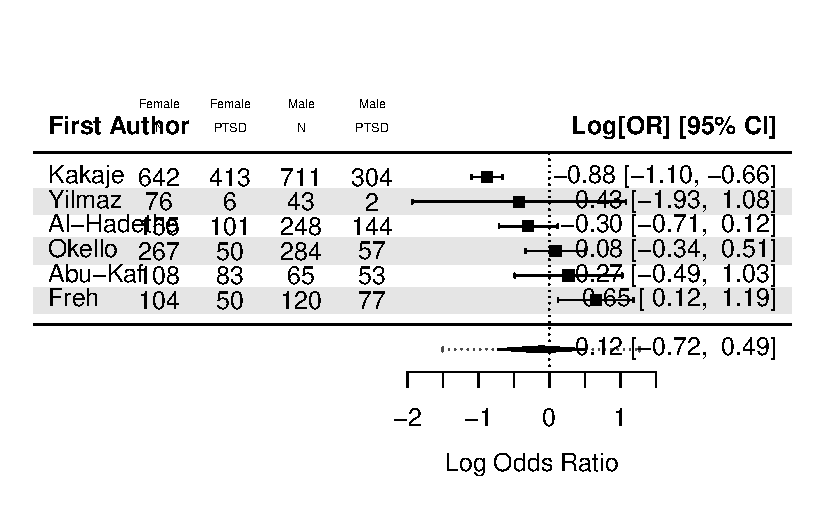
\includegraphics{1_descriptive_stats_files/figure-pdf/unnamed-chunk-15-1.pdf}

The above effect is negative, which here indicates that PTSD rates are
slightly here in women across the studies, but the effect is not
significant.

\subsection{R3) Meta-Regressions - age, ongoing war, method of
measurement, country income level (IN
PROGRESS)}\label{r3-meta-regressions---age-ongoing-war-method-of-measurement-country-income-level-in-progress}

\begin{Shaded}
\begin{Highlighting}[]
\CommentTok{\#| echo: true}
\CommentTok{\#| output: false}
\CommentTok{\#| warning: false}
\CommentTok{\#|}
\NormalTok{moderation\_models }\OtherTok{=} \FunctionTok{list}\NormalTok{()}

\NormalTok{moderation\_models[[}\StringTok{"Age"}\NormalTok{]] }\OtherTok{=} \FunctionTok{rma.glmm}\NormalTok{(}
  \AttributeTok{xi =} \StringTok{\textasciigrave{}}\AttributeTok{ptsd\_n}\StringTok{\textasciigrave{}}\NormalTok{, }
  \AttributeTok{ni =} \StringTok{\textasciigrave{}}\AttributeTok{participants}\StringTok{\textasciigrave{}}\NormalTok{, }
  \AttributeTok{data =}\NormalTok{ df, }
  \AttributeTok{measure=}\StringTok{"PLO"}\NormalTok{,}
  \AttributeTok{verbose =} \ConstantTok{FALSE}\NormalTok{,}
  \AttributeTok{method =} \StringTok{"ML"}\NormalTok{,}
  \CommentTok{\# intercept = FALSE,}
  \AttributeTok{mods =} \SpecialCharTok{\textasciitilde{}} \DecValTok{1} \SpecialCharTok{+}\NormalTok{ age\_centered,}
  \AttributeTok{to =} \StringTok{"all"}\NormalTok{,}
  \AttributeTok{test =} \StringTok{"t"} \CommentTok{\# This is recommended here metafor/html/misc{-}recs.html}
\NormalTok{)}

\NormalTok{moderation\_models[[}\StringTok{"War"}\NormalTok{]] }\OtherTok{=} \FunctionTok{rma.glmm}\NormalTok{(}
  \AttributeTok{xi =} \StringTok{\textasciigrave{}}\AttributeTok{ptsd\_n}\StringTok{\textasciigrave{}}\NormalTok{, }
  \AttributeTok{ni =} \StringTok{\textasciigrave{}}\AttributeTok{participants}\StringTok{\textasciigrave{}}\NormalTok{, }
  \AttributeTok{data =}\NormalTok{ df, }
  \AttributeTok{measure=}\StringTok{"PLO"}\NormalTok{,}
  \AttributeTok{verbose =} \ConstantTok{FALSE}\NormalTok{,}
  \AttributeTok{method =} \StringTok{"ML"}\NormalTok{,}
  \CommentTok{\# intercept = FALSE,}
  \AttributeTok{mods =} \SpecialCharTok{\textasciitilde{}} \DecValTok{1} \SpecialCharTok{+}\NormalTok{ war,}
  \AttributeTok{to =} \StringTok{"all"}\NormalTok{,}
  \AttributeTok{test =} \StringTok{"t"} \CommentTok{\# This is recommended here metafor/html/misc{-}recs.html}
\NormalTok{)}

\NormalTok{moderation\_models[[}\StringTok{"Aftermath"}\NormalTok{]] }\OtherTok{=} \FunctionTok{rma.glmm}\NormalTok{(}
  \AttributeTok{xi =} \StringTok{\textasciigrave{}}\AttributeTok{ptsd\_n}\StringTok{\textasciigrave{}}\NormalTok{, }
  \AttributeTok{ni =} \StringTok{\textasciigrave{}}\AttributeTok{participants}\StringTok{\textasciigrave{}}\NormalTok{, }
  \AttributeTok{data =}\NormalTok{ df, }
  \AttributeTok{measure=}\StringTok{"PLO"}\NormalTok{,}
  \AttributeTok{verbose =} \ConstantTok{FALSE}\NormalTok{,}
  \AttributeTok{method =} \StringTok{"ML"}\NormalTok{,}
  \CommentTok{\# intercept = FALSE,}
  \AttributeTok{mods =} \SpecialCharTok{\textasciitilde{}} \DecValTok{1} \SpecialCharTok{+}\NormalTok{ aftermath\_centered,}
  \AttributeTok{to =} \StringTok{"all"}\NormalTok{,}
  \AttributeTok{test =} \StringTok{"t"} \CommentTok{\# This is recommended here metafor/html/misc{-}recs.html}
\NormalTok{)}
\end{Highlighting}
\end{Shaded}

\begin{verbatim}
Warning: 9 studies with NAs omitted from model fitting.
\end{verbatim}

\begin{verbatim}
Warning: Some yi/vi values are NA.
\end{verbatim}

\begin{Shaded}
\begin{Highlighting}[]
\NormalTok{moderation\_models[[}\StringTok{"Measure"}\NormalTok{]] }\OtherTok{=} \FunctionTok{rma.glmm}\NormalTok{(}
  \AttributeTok{xi =} \StringTok{\textasciigrave{}}\AttributeTok{ptsd\_n}\StringTok{\textasciigrave{}}\NormalTok{, }
  \AttributeTok{ni =} \StringTok{\textasciigrave{}}\AttributeTok{participants}\StringTok{\textasciigrave{}}\NormalTok{, }
  \AttributeTok{data =}\NormalTok{ df, }
  \AttributeTok{measure=}\StringTok{"PLO"}\NormalTok{,}
  \AttributeTok{verbose =} \ConstantTok{FALSE}\NormalTok{,}
  \AttributeTok{method =} \StringTok{"ML"}\NormalTok{,}
  \CommentTok{\# intercept = FALSE,}
  \AttributeTok{mods =} \SpecialCharTok{\textasciitilde{}} \DecValTok{1} \SpecialCharTok{+}\NormalTok{ measure,}
  \AttributeTok{to =} \StringTok{"all"}\NormalTok{,}
  \AttributeTok{test =} \StringTok{"t"} \CommentTok{\# This is recommended here metafor/html/misc{-}recs.html}
\NormalTok{)}

\NormalTok{moderation\_models[[}\StringTok{"Economic"}\NormalTok{]] }\OtherTok{=} \FunctionTok{rma.glmm}\NormalTok{(}
  \AttributeTok{xi =} \StringTok{\textasciigrave{}}\AttributeTok{ptsd\_n}\StringTok{\textasciigrave{}}\NormalTok{, }
  \AttributeTok{ni =} \StringTok{\textasciigrave{}}\AttributeTok{participants}\StringTok{\textasciigrave{}}\NormalTok{, }
  \AttributeTok{data =}\NormalTok{ df, }
  \AttributeTok{measure=}\StringTok{"PLO"}\NormalTok{,}
  \AttributeTok{verbose =} \ConstantTok{FALSE}\NormalTok{,}
  \AttributeTok{method =} \StringTok{"ML"}\NormalTok{,}
  \CommentTok{\# intercept = FALSE,}
  \AttributeTok{mods =} \SpecialCharTok{\textasciitilde{}} \DecValTok{1} \SpecialCharTok{+} \FunctionTok{factor}\NormalTok{(econindex),}
  \AttributeTok{to =} \StringTok{"all"}\NormalTok{,}
  \AttributeTok{test =} \StringTok{"t"} \CommentTok{\# This is recommended here metafor/html/misc{-}recs.html}
\NormalTok{)}

\NormalTok{moderation\_models[[}\StringTok{"Quality"}\NormalTok{]] }\OtherTok{=} \FunctionTok{rma.glmm}\NormalTok{(}
  \AttributeTok{xi =} \StringTok{\textasciigrave{}}\AttributeTok{ptsd\_n}\StringTok{\textasciigrave{}}\NormalTok{, }
  \AttributeTok{ni =} \StringTok{\textasciigrave{}}\AttributeTok{participants}\StringTok{\textasciigrave{}}\NormalTok{, }
  \AttributeTok{data =}\NormalTok{ df, }
  \AttributeTok{measure=}\StringTok{"PLO"}\NormalTok{,}
  \AttributeTok{verbose =} \ConstantTok{FALSE}\NormalTok{,}
  \AttributeTok{method =} \StringTok{"ML"}\NormalTok{,}
  \CommentTok{\# intercept = FALSE,}
  \AttributeTok{mods =} \SpecialCharTok{\textasciitilde{}} \DecValTok{1} \SpecialCharTok{+}\NormalTok{ qualityassessment\_factor,}
  \AttributeTok{to =} \StringTok{"all"}\NormalTok{,}
  \AttributeTok{test =} \StringTok{"t"} \CommentTok{\# This is recommended here metafor/html/misc{-}recs.html}
\NormalTok{)}

\NormalTok{moderation\_models\_nointercept }\OtherTok{=} \FunctionTok{list}\NormalTok{()}

\NormalTok{moderation\_models\_nointercept[[}\StringTok{"Age"}\NormalTok{]] }\OtherTok{=} \FunctionTok{rma.glmm}\NormalTok{(}
  \AttributeTok{xi =} \StringTok{\textasciigrave{}}\AttributeTok{ptsd\_n}\StringTok{\textasciigrave{}}\NormalTok{, }
  \AttributeTok{ni =} \StringTok{\textasciigrave{}}\AttributeTok{participants}\StringTok{\textasciigrave{}}\NormalTok{, }
  \AttributeTok{data =}\NormalTok{ df, }
  \AttributeTok{measure=}\StringTok{"PLO"}\NormalTok{,}
  \AttributeTok{verbose =} \ConstantTok{FALSE}\NormalTok{,}
  \AttributeTok{method =} \StringTok{"ML"}\NormalTok{,}
  \CommentTok{\# intercept = FALSE,}
  \AttributeTok{mods =} \SpecialCharTok{\textasciitilde{}} \DecValTok{1} \SpecialCharTok{+}\NormalTok{ age\_centered,}
  \AttributeTok{to =} \StringTok{"all"}\NormalTok{,}
  \AttributeTok{test =} \StringTok{"t"} \CommentTok{\# This is recommended here metafor/html/misc{-}recs.html}
\NormalTok{)}

\NormalTok{moderation\_models\_nointercept[[}\StringTok{"War"}\NormalTok{]] }\OtherTok{=} \FunctionTok{rma.glmm}\NormalTok{(}
  \AttributeTok{xi =} \StringTok{\textasciigrave{}}\AttributeTok{ptsd\_n}\StringTok{\textasciigrave{}}\NormalTok{, }
  \AttributeTok{ni =} \StringTok{\textasciigrave{}}\AttributeTok{participants}\StringTok{\textasciigrave{}}\NormalTok{, }
  \AttributeTok{data =}\NormalTok{ df, }
  \AttributeTok{measure=}\StringTok{"PLO"}\NormalTok{,}
  \AttributeTok{verbose =} \ConstantTok{FALSE}\NormalTok{,}
  \AttributeTok{method =} \StringTok{"ML"}\NormalTok{,}
  \CommentTok{\# intercept = FALSE,}
  \AttributeTok{mods =} \SpecialCharTok{\textasciitilde{}} \DecValTok{0} \SpecialCharTok{+} \FunctionTok{factor}\NormalTok{(war),}
  \AttributeTok{to =} \StringTok{"all"}\NormalTok{,}
  \AttributeTok{test =} \StringTok{"t"} \CommentTok{\# This is recommended here metafor/html/misc{-}recs.html}
\NormalTok{)}

\NormalTok{moderation\_models\_nointercept[[}\StringTok{"Aftermath"}\NormalTok{]] }\OtherTok{=} \FunctionTok{rma.glmm}\NormalTok{(}
  \AttributeTok{xi =} \StringTok{\textasciigrave{}}\AttributeTok{ptsd\_n}\StringTok{\textasciigrave{}}\NormalTok{, }
  \AttributeTok{ni =} \StringTok{\textasciigrave{}}\AttributeTok{participants}\StringTok{\textasciigrave{}}\NormalTok{, }
  \AttributeTok{data =}\NormalTok{ df, }
  \AttributeTok{measure=}\StringTok{"PLO"}\NormalTok{,}
  \AttributeTok{verbose =} \ConstantTok{FALSE}\NormalTok{,}
  \AttributeTok{method =} \StringTok{"ML"}\NormalTok{,}
  \CommentTok{\# intercept = FALSE,}
  \AttributeTok{mods =} \SpecialCharTok{\textasciitilde{}} \DecValTok{1} \SpecialCharTok{+}\NormalTok{ aftermath\_centered,}
  \AttributeTok{to =} \StringTok{"all"}\NormalTok{,}
  \AttributeTok{test =} \StringTok{"t"} \CommentTok{\# This is recommended here metafor/html/misc{-}recs.html}
\NormalTok{)}
\end{Highlighting}
\end{Shaded}

\begin{verbatim}
Warning: 9 studies with NAs omitted from model fitting.

Warning: Some yi/vi values are NA.
\end{verbatim}

\begin{Shaded}
\begin{Highlighting}[]
\NormalTok{moderation\_models\_nointercept[[}\StringTok{"Measure"}\NormalTok{]] }\OtherTok{=} \FunctionTok{rma.glmm}\NormalTok{(}
  \AttributeTok{xi =} \StringTok{\textasciigrave{}}\AttributeTok{ptsd\_n}\StringTok{\textasciigrave{}}\NormalTok{, }
  \AttributeTok{ni =} \StringTok{\textasciigrave{}}\AttributeTok{participants}\StringTok{\textasciigrave{}}\NormalTok{, }
  \AttributeTok{data =}\NormalTok{ df, }
  \AttributeTok{measure=}\StringTok{"PLO"}\NormalTok{,}
  \AttributeTok{verbose =} \ConstantTok{FALSE}\NormalTok{,}
  \AttributeTok{method =} \StringTok{"ML"}\NormalTok{,}
  \CommentTok{\# intercept = FALSE,}
  \AttributeTok{mods =} \SpecialCharTok{\textasciitilde{}} \DecValTok{0} \SpecialCharTok{+}\NormalTok{ measure,}
  \AttributeTok{to =} \StringTok{"all"}\NormalTok{,}
  \AttributeTok{test =} \StringTok{"t"} \CommentTok{\# This is recommended here metafor/html/misc{-}recs.html}
\NormalTok{)}

\NormalTok{moderation\_models\_nointercept[[}\StringTok{"Economic"}\NormalTok{]] }\OtherTok{=} \FunctionTok{rma.glmm}\NormalTok{(}
  \AttributeTok{xi =} \StringTok{\textasciigrave{}}\AttributeTok{ptsd\_n}\StringTok{\textasciigrave{}}\NormalTok{, }
  \AttributeTok{ni =} \StringTok{\textasciigrave{}}\AttributeTok{participants}\StringTok{\textasciigrave{}}\NormalTok{, }
  \AttributeTok{data =}\NormalTok{ df, }
  \AttributeTok{measure=}\StringTok{"PLO"}\NormalTok{,}
  \AttributeTok{verbose =} \ConstantTok{FALSE}\NormalTok{,}
  \AttributeTok{method =} \StringTok{"ML"}\NormalTok{,}
  \CommentTok{\# intercept = FALSE,}
  \AttributeTok{mods =} \SpecialCharTok{\textasciitilde{}} \DecValTok{0} \SpecialCharTok{+} \FunctionTok{factor}\NormalTok{(econindex),}
  \AttributeTok{to =} \StringTok{"all"}\NormalTok{,}
  \AttributeTok{test =} \StringTok{"t"} \CommentTok{\# This is recommended here metafor/html/misc{-}recs.html}
\NormalTok{)}

\NormalTok{moderation\_models\_nointercept[[}\StringTok{"Quality"}\NormalTok{]] }\OtherTok{=} \FunctionTok{rma.glmm}\NormalTok{(}
  \AttributeTok{xi =} \StringTok{\textasciigrave{}}\AttributeTok{ptsd\_n}\StringTok{\textasciigrave{}}\NormalTok{, }
  \AttributeTok{ni =} \StringTok{\textasciigrave{}}\AttributeTok{participants}\StringTok{\textasciigrave{}}\NormalTok{, }
  \AttributeTok{data =}\NormalTok{ df, }
  \AttributeTok{measure=}\StringTok{"PLO"}\NormalTok{,}
  \AttributeTok{verbose =} \ConstantTok{FALSE}\NormalTok{,}
  \AttributeTok{method =} \StringTok{"ML"}\NormalTok{,}
  \CommentTok{\# intercept = FALSE,}
  \AttributeTok{mods =} \SpecialCharTok{\textasciitilde{}} \DecValTok{0} \SpecialCharTok{+}\NormalTok{ qualityassessment\_factor,}
  \AttributeTok{to =} \StringTok{"all"}\NormalTok{,}
  \AttributeTok{test =} \StringTok{"t"} \CommentTok{\# This is recommended here metafor/html/misc{-}recs.html}
\NormalTok{)}
\end{Highlighting}
\end{Shaded}

\subsubsection{Create Table}\label{create-table}

\begin{Shaded}
\begin{Highlighting}[]
\CommentTok{\# moderation\_models[[2]]}

\NormalTok{moderation\_results }\OtherTok{=} \FunctionTok{list}\NormalTok{()}

\ControlFlowTok{for}\NormalTok{ (i }\ControlFlowTok{in} \DecValTok{1}\SpecialCharTok{:}\FunctionTok{length}\NormalTok{(moderation\_models))\{}
\NormalTok{  moderation\_results[[i]] }\OtherTok{=} \FunctionTok{list}\NormalTok{()}
\NormalTok{  moderation\_results[[i]][[}\StringTok{"QM"}\NormalTok{]]    }\OtherTok{=}\NormalTok{ moderation\_models[[i]]}\SpecialCharTok{$}\NormalTok{QM}
\NormalTok{  moderation\_results[[i]][[}\StringTok{"QMdf\_1"}\NormalTok{]]  }\OtherTok{=}\NormalTok{ moderation\_models[[i]]}\SpecialCharTok{$}\NormalTok{QMdf[}\DecValTok{1}\NormalTok{]}
\NormalTok{  moderation\_results[[i]][[}\StringTok{"QMdf\_2"}\NormalTok{]]  }\OtherTok{=}\NormalTok{ moderation\_models[[i]]}\SpecialCharTok{$}\NormalTok{QMdf[}\DecValTok{2}\NormalTok{]}
\NormalTok{  moderation\_results[[i]][[}\StringTok{"QMp"}\NormalTok{]]   }\OtherTok{=}\NormalTok{ moderation\_models[[i]]}\SpecialCharTok{$}\NormalTok{QMp}
\NormalTok{  moderation\_results[[i]][[}\StringTok{"N Studies"}\NormalTok{]] }\OtherTok{=}  \FunctionTok{length}\NormalTok{(moderation\_models[[i]]}\SpecialCharTok{$}\NormalTok{ni)}
\NormalTok{  moderation\_results[[i]][[}\StringTok{"N Participants"}\NormalTok{]] }\OtherTok{=} \FunctionTok{sum}\NormalTok{(moderation\_models[[i]]}\SpecialCharTok{$}\NormalTok{ni)}
\NormalTok{\}}

\NormalTok{moderation\_df }\OtherTok{\textless{}{-}} \FunctionTok{do.call}\NormalTok{(rbind, }\FunctionTok{lapply}\NormalTok{(moderation\_results, }\ControlFlowTok{function}\NormalTok{(x) }\FunctionTok{as.data.frame}\NormalTok{(}\FunctionTok{t}\NormalTok{(}\FunctionTok{unlist}\NormalTok{(x)))))}

\FunctionTok{rownames}\NormalTok{(moderation\_df) }\OtherTok{=} \FunctionTok{names}\NormalTok{(moderation\_models)}

\NormalTok{moderation\_df }\SpecialCharTok{\%\textgreater{}\%}
  \FunctionTok{gt}\NormalTok{(}\AttributeTok{rowname\_col =} \StringTok{"Moderation Test"}\NormalTok{,}
     \AttributeTok{rownames\_to\_stub =} \ConstantTok{TRUE}\NormalTok{) }\SpecialCharTok{\%\textgreater{}\%}
\NormalTok{  gt}\SpecialCharTok{::}\FunctionTok{tab\_header}\NormalTok{(}\AttributeTok{title =} \StringTok{"Moderation Tests"}\NormalTok{) }\SpecialCharTok{\%\textgreater{}\%}
  \FunctionTok{fmt\_number}\NormalTok{(}\AttributeTok{columns =} \FunctionTok{c}\NormalTok{(QM,QMp), }\AttributeTok{decimals =} \DecValTok{3}\NormalTok{)}
\end{Highlighting}
\end{Shaded}

\begin{longtable*}{l|rrrrrr}
\caption*{
{\large Moderation Tests}
} \\ 
\toprule
\multicolumn{1}{l}{} & QM & QMdf\_1 & QMdf\_2 & QMp & N Studies & N Participants \\ 
\midrule\addlinespace[2.5pt]
Age & $2.654$ & 1 & 19 & $0.120$ & 21 & 12914 \\ 
War & $0.100$ & 1 & 19 & $0.755$ & 21 & 12914 \\ 
Aftermath & $8.749$ & 1 & 10 & $0.014$ & 12 & 7532 \\ 
Measure & $6.499$ & 11 & 9 & $0.005$ & 21 & 12914 \\ 
Economic & $0.173$ & 3 & 17 & $0.913$ & 21 & 12914 \\ 
Quality & $1.695$ & 6 & 14 & $0.195$ & 21 & 12914 \\ 
\bottomrule
\end{longtable*}

\begin{Shaded}
\begin{Highlighting}[]
\NormalTok{moderation\_coef }\OtherTok{=} \FunctionTok{list}\NormalTok{()}

\ControlFlowTok{for}\NormalTok{ (i }\ControlFlowTok{in} \DecValTok{1}\SpecialCharTok{:}\FunctionTok{length}\NormalTok{(moderation\_models\_nointercept))\{}
\NormalTok{  moderation\_coef[[i]]          }\OtherTok{=} \FunctionTok{list}\NormalTok{()}
\NormalTok{  moderation\_coef[[i]][[}\StringTok{"QM"}\NormalTok{]]  }\OtherTok{=}\NormalTok{ moderation\_models\_nointercept[[i]]}
  
\NormalTok{  moderation\_coef[[i]] }\OtherTok{=} \FunctionTok{data.frame}\NormalTok{(}
    \AttributeTok{model =} \FunctionTok{names}\NormalTok{(moderation\_models\_nointercept)[i],}
    \AttributeTok{group =} \FunctionTok{rownames}\NormalTok{(moderation\_models\_nointercept[[i]]}\SpecialCharTok{$}\NormalTok{beta),}
    \AttributeTok{b     =}\NormalTok{ moderation\_models\_nointercept[[i]][}\FunctionTok{c}\NormalTok{(}\StringTok{"b"}\NormalTok{)],}
    \AttributeTok{ci.lb =}\NormalTok{ moderation\_models\_nointercept[[i]][}\FunctionTok{c}\NormalTok{(}\StringTok{"ci.lb"}\NormalTok{)],}
    \AttributeTok{ci.ub =}\NormalTok{ moderation\_models\_nointercept[[i]][}\FunctionTok{c}\NormalTok{(}\StringTok{"ci.ub"}\NormalTok{)],}
    \AttributeTok{se    =}\NormalTok{ moderation\_models\_nointercept[[i]][}\FunctionTok{c}\NormalTok{(}\StringTok{"se"}\NormalTok{)],}
    \AttributeTok{p     =}\NormalTok{ moderation\_models\_nointercept[[i]][}\FunctionTok{c}\NormalTok{(}\StringTok{"pval"}\NormalTok{)]}
\NormalTok{  )}
  
   \CommentTok{\# moderation\_coef[[i]] = moderation\_coef[[i]] \%\textgreater{}\%}
   \CommentTok{\#   mutate(across(c(b, ci.lb, ci.ub), \textasciitilde{}plogis(.x)))}
  
\NormalTok{\}}

\NormalTok{moderation\_coef[[}\FunctionTok{match}\NormalTok{(}\StringTok{"War"}\NormalTok{, }\FunctionTok{names}\NormalTok{(moderation\_models))]]}\SpecialCharTok{$}\NormalTok{group }\OtherTok{=} \FunctionTok{c}\NormalTok{(}\StringTok{"Ongoing War"}\NormalTok{,}\StringTok{"Aftermath"}\NormalTok{)}

\NormalTok{moderation\_coef }\SpecialCharTok{\%\textgreater{}\%}
  \FunctionTok{do.call}\NormalTok{(}\StringTok{"bind\_rows"}\NormalTok{,.) }\SpecialCharTok{\%\textgreater{}\%}
  \StringTok{\textasciigrave{}}\AttributeTok{rownames\textless{}{-}}\StringTok{\textasciigrave{}}\NormalTok{((}\ConstantTok{NULL}\NormalTok{)) }\SpecialCharTok{\%\textgreater{}\%}
  \FunctionTok{select}\NormalTok{(}\SpecialCharTok{{-}}\NormalTok{pval) }\SpecialCharTok{\%\textgreater{}\%}
  \FunctionTok{select}\NormalTok{(}\SpecialCharTok{{-}}\NormalTok{se) }\SpecialCharTok{\%\textgreater{}\%}
  \FunctionTok{mutate}\NormalTok{(}\AttributeTok{group =} \FunctionTok{gsub}\NormalTok{(}\StringTok{"measure"}\NormalTok{,}\StringTok{""}\NormalTok{, group)) }\SpecialCharTok{\%\textgreater{}\%}
  \FunctionTok{mutate}\NormalTok{(}\AttributeTok{group =} \FunctionTok{gsub}\NormalTok{(}\StringTok{"factor}\SpecialCharTok{\textbackslash{}\textbackslash{}}\StringTok{(econindex}\SpecialCharTok{\textbackslash{}\textbackslash{}}\StringTok{)"}\NormalTok{,}\StringTok{""}\NormalTok{, group)) }\SpecialCharTok{\%\textgreater{}\%}
  \FunctionTok{mutate}\NormalTok{(}\AttributeTok{group =} \FunctionTok{gsub}\NormalTok{(}\StringTok{"qualityassessment\_factor"}\NormalTok{,}\StringTok{""}\NormalTok{, group)) }\SpecialCharTok{\%\textgreater{}\%}
  \FunctionTok{mutate}\NormalTok{(}\AttributeTok{group =} \FunctionTok{gsub}\NormalTok{(}\StringTok{"intrcpt"}\NormalTok{,}\StringTok{"Intercept"}\NormalTok{, group)) }\SpecialCharTok{\%\textgreater{}\%}
  \FunctionTok{gt}\NormalTok{() }\SpecialCharTok{\%\textgreater{}\%}
  \FunctionTok{cols\_hide}\NormalTok{(}\StringTok{"model"}\NormalTok{) }\SpecialCharTok{\%\textgreater{}\%}
  \FunctionTok{tab\_row\_group}\NormalTok{(}
    \AttributeTok{label =} \StringTok{"Ongoing / Aftermath War, F(df1 = 1, df2 = 19) = .43, p = .84"}\NormalTok{,}
    \AttributeTok{rows =} \FunctionTok{which}\NormalTok{(model}\SpecialCharTok{==}\StringTok{"War"}\NormalTok{)}
\NormalTok{  ) }\SpecialCharTok{\%\textgreater{}\%}
    \FunctionTok{tab\_row\_group}\NormalTok{(}
    \AttributeTok{label =} \StringTok{"Mean Sample Age, F(df1 = 1, df2 = 19) = 2.95, p = .10"}\NormalTok{,}
    \AttributeTok{rows =} \FunctionTok{which}\NormalTok{(model}\SpecialCharTok{==}\StringTok{"Age"}\NormalTok{)}
\NormalTok{  ) }\SpecialCharTok{\%\textgreater{}\%}
    \FunctionTok{tab\_row\_group}\NormalTok{(}
    \AttributeTok{label =} \StringTok{"PTSD Measure, F(df1 = 11, df2 = 9) = 5.64, p = .007"}\NormalTok{,}
    \AttributeTok{rows =} \FunctionTok{which}\NormalTok{(model}\SpecialCharTok{==}\StringTok{"Measure"}\NormalTok{)}
\NormalTok{  ) }\SpecialCharTok{\%\textgreater{}\%}
    \FunctionTok{tab\_row\_group}\NormalTok{(}
    \AttributeTok{label =} \StringTok{"Economic Index, F(df1 = 3, df2 = 17) = 0.21, p = .89"}\NormalTok{,}
    \AttributeTok{rows =} \FunctionTok{which}\NormalTok{(model}\SpecialCharTok{==}\StringTok{"Economic"}\NormalTok{)}
\NormalTok{  ) }\SpecialCharTok{\%\textgreater{}\%}
    \FunctionTok{tab\_row\_group}\NormalTok{(}
    \AttributeTok{label =} \StringTok{"Aftermath Length, F(df1 = 1, df2 = 10) = 8.75, p = .014"}\NormalTok{,}
    \AttributeTok{rows =} \FunctionTok{which}\NormalTok{(model}\SpecialCharTok{==}\StringTok{"Aftermath"}\NormalTok{)}
\NormalTok{  ) }\SpecialCharTok{\%\textgreater{}\%}
  \FunctionTok{tab\_row\_group}\NormalTok{(}
    \AttributeTok{label =} \StringTok{"Quality Assessment, F(df1 = 6, df2 = 14) = 1.87, p = .16"}\NormalTok{,}
    \AttributeTok{rows =} \FunctionTok{which}\NormalTok{(model}\SpecialCharTok{==}\StringTok{"Quality"}\NormalTok{)}
\NormalTok{  ) }\SpecialCharTok{\%\textgreater{}\%}
   \FunctionTok{fmt\_percent}\NormalTok{(}
    \AttributeTok{rows     =}\NormalTok{ (model }\SpecialCharTok{!=} \StringTok{"Age"}\NormalTok{) }\SpecialCharTok{\&}\NormalTok{ (model }\SpecialCharTok{!=} \StringTok{"Aftermath"}\NormalTok{),}
    \AttributeTok{columns  =} \FunctionTok{everything}\NormalTok{(),}
    \AttributeTok{decimals =} \DecValTok{1}\NormalTok{,}
    \AttributeTok{use\_seps =} \ConstantTok{FALSE}
\NormalTok{  ) }\SpecialCharTok{\%\textgreater{}\%}
  \FunctionTok{fmt}\NormalTok{(}
    \AttributeTok{rows     =}\NormalTok{ (model }\SpecialCharTok{!=} \StringTok{"Age"}\NormalTok{) }\SpecialCharTok{|}\NormalTok{ (model }\SpecialCharTok{!=} \StringTok{"Aftermath"}\NormalTok{),}
    \AttributeTok{columns  =} \FunctionTok{c}\NormalTok{(b, ci.lb, ci.ub),}
    \AttributeTok{fns      =} \ControlFlowTok{function}\NormalTok{(x) \{}\FunctionTok{paste0}\NormalTok{(}\FunctionTok{signif}\NormalTok{((}\FunctionTok{plogis}\NormalTok{(x)}\SpecialCharTok{*}\DecValTok{100}\NormalTok{),}\DecValTok{3}\NormalTok{),}\StringTok{"\%"}\NormalTok{)\}}
\NormalTok{  ) }\SpecialCharTok{\%\textgreater{}\%}
   \FunctionTok{fmt}\NormalTok{(}
    \AttributeTok{rows     =}\NormalTok{ (model }\SpecialCharTok{==} \StringTok{"Age"}\NormalTok{) }\SpecialCharTok{|}\NormalTok{ (model }\SpecialCharTok{==} \StringTok{"Aftermath"}\NormalTok{),}
    \AttributeTok{columns  =} \FunctionTok{c}\NormalTok{(b, ci.lb, ci.ub),}
    \AttributeTok{fns      =} \ControlFlowTok{function}\NormalTok{(x) \{}\FunctionTok{paste0}\NormalTok{(}\StringTok{"b = "}\NormalTok{, gbtoolbox}\SpecialCharTok{::}\FunctionTok{apa\_num}\NormalTok{(}\FunctionTok{as.numeric}\NormalTok{(x)))\}}
\NormalTok{  )}
\end{Highlighting}
\end{Shaded}

\begin{longtable*}{lrrr}
\toprule
group & b & ci.lb & ci.ub \\ 
\midrule\addlinespace[2.5pt]
\multicolumn{4}{l}{Quality Assessment, F(df1 = 6, df2 = 14) = 1.87, p = .16} \\ 
\midrule\addlinespace[2.5pt]
Quality Rating: 1 & 79.4% & 27.8% & 97.5% \\ 
Quality Rating: 3 & 13.9% & 4.76% & 34.4% \\ 
Quality Rating: 4 & 45% & 14% & 80.4% \\ 
Quality Rating: 5 & 46.2% & 8.08% & 89.3% \\ 
Quality Rating: 6 & 37.7% & 14% & 69.2% \\ 
Quality Rating: 7 & 31.7% & 15.4% & 54.2% \\ 
Quality Rating: 9 & 18.8% & 6.79% & 42.3% \\ 
\midrule\addlinespace[2.5pt]
\multicolumn{4}{l}{Aftermath Length, F(df1 = 1, df2 = 10) = 8.75, p = .014} \\ 
\midrule\addlinespace[2.5pt]
Intercept & b = -.95 & b = -1.68 & b = -.23 \\ 
aftermath\_centered & b =  .25 & b =  .06 & b =  .45 \\ 
\midrule\addlinespace[2.5pt]
\multicolumn{4}{l}{Economic Index, F(df1 = 3, df2 = 17) = 0.21, p = .89} \\ 
\midrule\addlinespace[2.5pt]
1 & 27.9% & 11.2% & 54.2% \\ 
2 & 29.9% & 9.96% & 62.3% \\ 
3 & 40.1% & 12.2% & 76.4% \\ 
4 & 26.6% & 12.2% & 48.7% \\ 
\midrule\addlinespace[2.5pt]
\multicolumn{4}{l}{PTSD Measure, F(df1 = 11, df2 = 9) = 5.64, p = .007} \\ 
\midrule\addlinespace[2.5pt]
CBCL & 79.3% & 49.3% & 93.8% \\ 
CPSS & 2.04% & 0.39% & 9.98% \\ 
CPTS-RI & 15% & 4.52% & 39.6% \\ 
CRIES & 43.7% & 28.1% & 60.7% \\ 
DSM-5 & 6.47% & 1.44% & 24.7% \\ 
HTQ & 5.3% & 1.45% & 17.5% \\ 
IES-R & 34.1% & 16.8% & 56.8% \\ 
PCL-5 & 49.8% & 21% & 78.8% \\ 
PCL-C & 12.5% & 3.16% & 38.3% \\ 
PTSDSS & 54.7% & 32% & 75.5% \\ 
SPTSS & 61.1% & 29.4% & 85.6% \\ 
UCLA-PTS & 26.2% & 16.3% & 39.3% \\ 
\midrule\addlinespace[2.5pt]
\multicolumn{4}{l}{Mean Sample Age, F(df1 = 1, df2 = 19) = 2.95, p = .10} \\ 
\midrule\addlinespace[2.5pt]
Intercept & b = -.88 & b = -1.44 & b = -.32 \\ 
age\_centered & b =  .26 & b = -.07 & b =  .59 \\ 
\midrule\addlinespace[2.5pt]
\multicolumn{4}{l}{Ongoing / Aftermath War, F(df1 = 1, df2 = 19) = .43, p = .84} \\ 
\midrule\addlinespace[2.5pt]
Ongoing War & 31.6% & 15.7% & 53.4% \\ 
Aftermath & 27.8% & 14.9% & 45.8% \\ 
\bottomrule
\end{longtable*}

\subsubsection{Additional Plots}\label{additional-plots}

\subsubsection{Age}\label{age}

\begin{Shaded}
\begin{Highlighting}[]
\NormalTok{df }\SpecialCharTok{\%\textgreater{}\%}
  \FunctionTok{arrange}\NormalTok{((prev\_plo\_var))}\SpecialCharTok{\%\textgreater{}\%}
  \FunctionTok{mutate}\NormalTok{(}\AttributeTok{war\_factor =} \FunctionTok{factor}\NormalTok{(war, }\AttributeTok{levels =} \DecValTok{0}\SpecialCharTok{:}\DecValTok{1}\NormalTok{, }\AttributeTok{labels =} \FunctionTok{c}\NormalTok{(}\StringTok{"On Going"}\NormalTok{, }\StringTok{"Aftermath"}\NormalTok{)),}
         \AttributeTok{war\_factor =}\NormalTok{ forcats}\SpecialCharTok{::}\FunctionTok{fct\_explicit\_na}\NormalTok{(war\_factor, }\AttributeTok{na\_level =} \StringTok{"Missing"}\NormalTok{)) }\SpecialCharTok{\%\textgreater{}\%}
  \FunctionTok{ggplot}\NormalTok{(}\FunctionTok{aes}\NormalTok{(}\AttributeTok{y =}\NormalTok{ prev\_pr, }\AttributeTok{x =}\NormalTok{ age)) }\SpecialCharTok{+}
  \FunctionTok{geom\_point}\NormalTok{(}\FunctionTok{aes}\NormalTok{(}\AttributeTok{size =} \DecValTok{1}\SpecialCharTok{/}\NormalTok{prev\_plo\_var, }\AttributeTok{shape =}\NormalTok{ war\_factor,}\AttributeTok{col =}\NormalTok{ war\_factor)) }\SpecialCharTok{+} 
  \FunctionTok{labs}\NormalTok{(}\AttributeTok{x =} \StringTok{"Mean Sample Age (Years)"}\NormalTok{, }\AttributeTok{y =} \StringTok{"PTSD Prevalence"}\NormalTok{,}
       \AttributeTok{col =} \StringTok{"War"}\NormalTok{, }\AttributeTok{shape =} \StringTok{"War"}\NormalTok{) }\SpecialCharTok{+}
\NormalTok{  ggrepel}\SpecialCharTok{::}\FunctionTok{geom\_text\_repel}\NormalTok{(}\FunctionTok{aes}\NormalTok{(}\AttributeTok{label =}\NormalTok{ authors), }\AttributeTok{size =} \DecValTok{3}\NormalTok{) }\SpecialCharTok{+}
  \FunctionTok{guides}\NormalTok{(}\AttributeTok{size =} \StringTok{"none"}\NormalTok{) }
\end{Highlighting}
\end{Shaded}

\begin{verbatim}
Warning: There was 1 warning in `mutate()`.
i In argument: `war_factor = forcats::fct_explicit_na(war_factor, na_level =
  "Missing")`.
Caused by warning:
! `fct_explicit_na()` was deprecated in forcats 1.0.0.
i Please use `fct_na_value_to_level()` instead.
\end{verbatim}

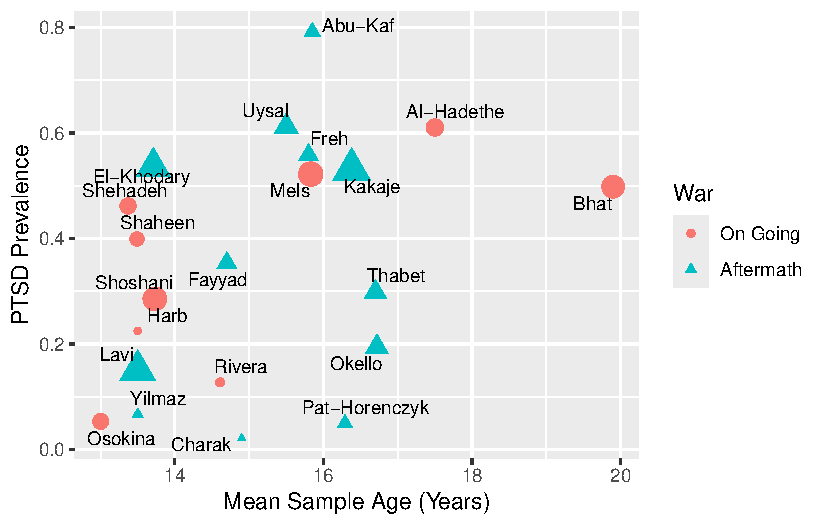
\includegraphics{1_descriptive_stats_files/figure-pdf/unnamed-chunk-19-1.pdf}

\begin{Shaded}
\begin{Highlighting}[]
  \FunctionTok{table}\NormalTok{(df}\SpecialCharTok{$}\NormalTok{war)}
\end{Highlighting}
\end{Shaded}

\begin{verbatim}

 0  1 
 9 12 
\end{verbatim}

\subsubsection{Aftermath}\label{aftermath}

\begin{Shaded}
\begin{Highlighting}[]
\NormalTok{intercept }\OtherTok{=}\NormalTok{ moderation\_models}\SpecialCharTok{$}\NormalTok{Aftermath}\SpecialCharTok{$}\NormalTok{b[}\DecValTok{1}\NormalTok{,}\DecValTok{1}\NormalTok{]}
\NormalTok{slope }\OtherTok{=}\NormalTok{ moderation\_models}\SpecialCharTok{$}\NormalTok{Aftermath}\SpecialCharTok{$}\NormalTok{b[}\DecValTok{2}\NormalTok{,}\DecValTok{1}\NormalTok{]}

\NormalTok{df }\SpecialCharTok{\%\textgreater{}\%}
  \FunctionTok{arrange}\NormalTok{((prev\_plo\_var))}\SpecialCharTok{\%\textgreater{}\%}
  \FunctionTok{filter}\NormalTok{(}\SpecialCharTok{!}\FunctionTok{is.na}\NormalTok{(aftermath)) }\SpecialCharTok{\%\textgreater{}\%}
  \FunctionTok{mutate}\NormalTok{(}\AttributeTok{war\_factor =} \FunctionTok{factor}\NormalTok{(war, }\AttributeTok{levels =} \DecValTok{0}\SpecialCharTok{:}\DecValTok{1}\NormalTok{, }\AttributeTok{labels =} \FunctionTok{c}\NormalTok{(}\StringTok{"On Going"}\NormalTok{, }\StringTok{"Aftermath"}\NormalTok{)),}
         \AttributeTok{war\_factor =}\NormalTok{ forcats}\SpecialCharTok{::}\FunctionTok{fct\_explicit\_na}\NormalTok{(war\_factor, }\AttributeTok{na\_level =} \StringTok{"Missing"}\NormalTok{)) }\SpecialCharTok{\%\textgreater{}\%}
  \FunctionTok{ggplot}\NormalTok{(}\FunctionTok{aes}\NormalTok{(}
    \AttributeTok{y =}\NormalTok{ prev\_pr, }
    \AttributeTok{x =}\NormalTok{ aftermath,}
    \AttributeTok{col =}\NormalTok{ authors}
\NormalTok{    )) }\SpecialCharTok{+}
  \FunctionTok{geom\_point}\NormalTok{(}
    \FunctionTok{aes}\NormalTok{(}
      \AttributeTok{size =} \DecValTok{1}\SpecialCharTok{/}\NormalTok{prev\_plo\_var}
\NormalTok{      )) }\SpecialCharTok{+} 
  \FunctionTok{labs}\NormalTok{(}
    \AttributeTok{x =} \StringTok{"Aftermath Length (Years)"}\NormalTok{, }
       \AttributeTok{y =} \StringTok{"PTSD Prevalence"}\NormalTok{,}
       \AttributeTok{col =} \StringTok{"War"}\NormalTok{, }
       \AttributeTok{shape =} \StringTok{"War"}
\NormalTok{    ) }\SpecialCharTok{+}
\NormalTok{  ggrepel}\SpecialCharTok{::}\FunctionTok{geom\_text\_repel}\NormalTok{(}
    \AttributeTok{seed =} \DecValTok{10}\NormalTok{,}
    \FunctionTok{aes}\NormalTok{(}
      \AttributeTok{label =}\NormalTok{ authors}
\NormalTok{      ), }
    \AttributeTok{size =} \DecValTok{3}
\NormalTok{    ) }\SpecialCharTok{+}
  \CommentTok{\# Note theat the analyses use aftermath centered, so we need to adjust for that here}
  \FunctionTok{geom\_function}\NormalTok{(}
    \AttributeTok{fun =} \ControlFlowTok{function}\NormalTok{(x) }\FunctionTok{plogis}\NormalTok{(intercept }\SpecialCharTok{+}\NormalTok{ slope}\SpecialCharTok{*}\NormalTok{(x }\SpecialCharTok{{-}} \FunctionTok{mean}\NormalTok{(df}\SpecialCharTok{$}\NormalTok{aftermath, }\AttributeTok{na.rm =} \ConstantTok{TRUE}\NormalTok{))), }
    \AttributeTok{colour =} \StringTok{"black"}\NormalTok{,}
    \AttributeTok{linewidth =} \DecValTok{1}
    \CommentTok{\# xlim = c({-}4,7)}
\NormalTok{    ) }\SpecialCharTok{+}
  \FunctionTok{guides}\NormalTok{(}\AttributeTok{size =} \StringTok{"none"}\NormalTok{, }\AttributeTok{col =} \StringTok{"none"}\NormalTok{) }\SpecialCharTok{+}
  \FunctionTok{scale\_y\_continuous}\NormalTok{(}
    \AttributeTok{breaks =}\NormalTok{ (}\FunctionTok{seq}\NormalTok{(}\DecValTok{0}\NormalTok{,}\DecValTok{1}\NormalTok{,}\AttributeTok{by=}\NormalTok{.}\DecValTok{1}\NormalTok{)), }\CommentTok{\# Labels for the ticks, in their original, untransformed units}
    \AttributeTok{labels =} \FunctionTok{paste0}\NormalTok{((}\DecValTok{0}\SpecialCharTok{:}\DecValTok{10}\NormalTok{)}\SpecialCharTok{*}\DecValTok{10}\NormalTok{,}\StringTok{"\%"}\NormalTok{)}
\NormalTok{  ) }\SpecialCharTok{+}
  \FunctionTok{scale\_color\_manual}\NormalTok{(}\AttributeTok{values =} \FunctionTok{c}\NormalTok{(}\StringTok{"\#E69F00"}\NormalTok{, }\StringTok{"\#56B4E9"}\NormalTok{, }\StringTok{"\#009E73"}\NormalTok{, }\StringTok{"\#0072B2"}\NormalTok{, }\StringTok{"\#0072B2"}\NormalTok{, }\StringTok{"\#D55E00"}\NormalTok{, }\StringTok{"\#CC79A7"}\NormalTok{, }\StringTok{"\#999999"}\NormalTok{, }\StringTok{"\#000000"}\NormalTok{, }\StringTok{"\#FFB000"}\NormalTok{, }\StringTok{"\#90B000"}\NormalTok{, }\StringTok{"\#B000B0"}\NormalTok{)) }\SpecialCharTok{+} 
  \FunctionTok{theme\_light}\NormalTok{()}
\end{Highlighting}
\end{Shaded}

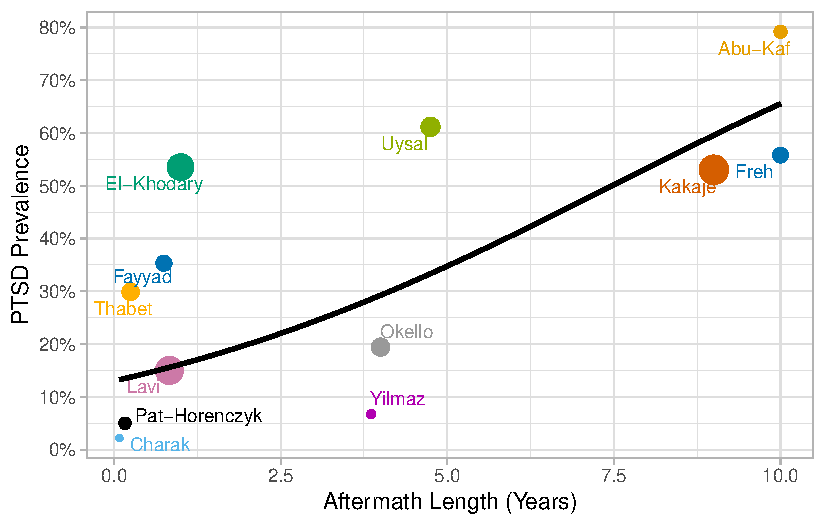
\includegraphics{1_descriptive_stats_files/figure-pdf/unnamed-chunk-20-1.pdf}

\begin{Shaded}
\begin{Highlighting}[]
\FunctionTok{ggsave}\NormalTok{(}\AttributeTok{file =} \FunctionTok{file.path}\NormalTok{(}\StringTok{"plots"}\NormalTok{,}\StringTok{"bubbleplot\_aftermath2.pdf"}\NormalTok{), }\AttributeTok{width =} \DecValTok{4}\NormalTok{, }\AttributeTok{height =} \DecValTok{4}\NormalTok{)}
\end{Highlighting}
\end{Shaded}

\subsection{Appendix: Model Output}\label{appendix-model-output}

Intercept models

\begin{Shaded}
\begin{Highlighting}[]
\NormalTok{moderation\_models}
\end{Highlighting}
\end{Shaded}

\begin{verbatim}
$Age

Mixed-Effects Model (k = 21; tau^2 estimator: ML)

tau^2 (estimated amount of residual heterogeneity):     1.4794
tau (square root of estimated tau^2 value):             1.2163
I^2 (residual heterogeneity / unaccounted variability): 99.33%
H^2 (unaccounted variability / sampling variability):   150.26

Tests for Residual Heterogeneity:
Wld(df = 19) = 1562.4196, p-val < .0001
LRT(df = 19) = 2117.5122, p-val < .0001

Test of Moderators (coefficient 2):
F(df1 = 1, df2 = 19) = 2.6540, p-val = 0.1198

Model Results:

              estimate      se     tval  df    pval    ci.lb    ci.ub     
intrcpt        -0.8787  0.2686  -3.2720  19  0.0040  -1.4409  -0.3166  ** 
age_centered    0.2563  0.1573   1.6291  19  0.1198  -0.0730   0.5856     

---
Signif. codes:  0 '***' 0.001 '**' 0.01 '*' 0.05 '.' 0.1 ' ' 1


$War

Mixed-Effects Model (k = 21; tau^2 estimator: ML)

tau^2 (estimated amount of residual heterogeneity):     1.6676
tau (square root of estimated tau^2 value):             1.2914
I^2 (residual heterogeneity / unaccounted variability): 99.41%
H^2 (unaccounted variability / sampling variability):   169.49

Tests for Residual Heterogeneity:
Wld(df = 19) = 1916.8994, p-val < .0001
LRT(df = 19) = 2737.3428, p-val < .0001

Test of Moderators (coefficient 2):
F(df1 = 1, df2 = 19) = 0.0999, p-val = 0.7554

Model Results:

         estimate      se     tval  df    pval    ci.lb   ci.ub    
intrcpt   -0.7739  0.4346  -1.7807  19  0.0910  -1.6836  0.1357  . 
war       -0.1818  0.5752  -0.3161  19  0.7554  -1.3858  1.0221    

---
Signif. codes:  0 '***' 0.001 '**' 0.01 '*' 0.05 '.' 0.1 ' ' 1


$Aftermath

Mixed-Effects Model (k = 12; tau^2 estimator: ML)

tau^2 (estimated amount of residual heterogeneity):     1.2281
tau (square root of estimated tau^2 value):             1.1082
I^2 (residual heterogeneity / unaccounted variability): 99.07%
H^2 (unaccounted variability / sampling variability):   107.33

Tests for Residual Heterogeneity:
Wld(df = 10) = 814.4552, p-val < .0001
LRT(df = 10) = 972.6039, p-val < .0001

Test of Moderators (coefficient 2):
F(df1 = 1, df2 = 10) = 8.7495, p-val = 0.0143

Model Results:

                    estimate      se     tval  df    pval    ci.lb    ci.ub    
intrcpt              -0.9534  0.3248  -2.9352  10  0.0149  -1.6771  -0.2297  * 
aftermath_centered    0.2543  0.0860   2.9580  10  0.0143   0.0627   0.4459  * 

---
Signif. codes:  0 '***' 0.001 '**' 0.01 '*' 0.05 '.' 0.1 ' ' 1


$Measure

Mixed-Effects Model (k = 21; tau^2 estimator: ML)

tau^2 (estimated amount of residual heterogeneity):     0.3343
tau (square root of estimated tau^2 value):             0.5782
I^2 (residual heterogeneity / unaccounted variability): 96.68%
H^2 (unaccounted variability / sampling variability):   30.08

Tests for Residual Heterogeneity:
Wld(df = 9) = 348.4233, p-val < .0001
LRT(df = 9) = 457.2590, p-val < .0001

Test of Moderators (coefficients 2:12):
F(df1 = 11, df2 = 9) = 6.4987, p-val = 0.0045

Model Results:

                 estimate      se     tval  df    pval    ci.lb    ci.ub      
intrcpt            1.3454  0.6081   2.2125   9  0.0542  -0.0302   2.7209    . 
measureCPSS       -5.2167  0.9572  -5.4497   9  0.0004  -7.3822  -3.0513  *** 
measureCPTS-RI    -3.0816  0.8411  -3.6638   9  0.0052  -4.9844  -1.1789   ** 
measureCRIES      -1.5973  0.6797  -2.3500   9  0.0433  -3.1349  -0.0597    * 
measureDSM-5      -4.0170  0.9178  -4.3769   9  0.0018  -6.0932  -1.9409   ** 
measureHTQ        -4.2278  0.8472  -4.9906   9  0.0007  -6.1442  -2.3114  *** 
measureIES-R      -2.0057  0.7354  -2.7274   9  0.0233  -3.6693  -0.3421    * 
measurePCL-5      -1.3527  0.8421  -1.6064   9  0.1427  -3.2576   0.5522      
measurePCL-C      -3.2948  0.8912  -3.6970   9  0.0049  -5.3109  -1.2787   ** 
measurePTSDSS     -1.1581  0.7364  -1.5725   9  0.1503  -2.8240   0.5079      
measureSPTSS      -0.8950  0.8453  -1.0588   9  0.3173  -2.8072   1.0172      
measureUCLA-PTS   -2.3789  0.6634  -3.5861   9  0.0059  -3.8795  -0.8782   ** 

---
Signif. codes:  0 '***' 0.001 '**' 0.01 '*' 0.05 '.' 0.1 ' ' 1


$Economic

Mixed-Effects Model (k = 21; tau^2 estimator: ML)

tau^2 (estimated amount of residual heterogeneity):     1.6317
tau (square root of estimated tau^2 value):             1.2774
I^2 (residual heterogeneity / unaccounted variability): 99.36%
H^2 (unaccounted variability / sampling variability):   155.09

Tests for Residual Heterogeneity:
Wld(df = 17) = 1606.0949, p-val < .0001
LRT(df = 17) = 2379.7443, p-val < .0001

Test of Moderators (coefficients 2:4):
F(df1 = 3, df2 = 17) = 0.1731, p-val = 0.9131

Model Results:

                    estimate      se     tval  df    pval    ci.lb   ci.ub    
intrcpt              -0.9506  0.5306  -1.7914  17  0.0911  -2.0701  0.1690  . 
factor(econindex)2    0.1005  0.8319   0.1208  17  0.9053  -1.6546  1.8555    
factor(econindex)3    0.5495  0.9153   0.6003  17  0.5562  -1.3816  2.4806    
factor(econindex)4   -0.0640  0.6994  -0.0915  17  0.9282  -1.5396  1.4116    

---
Signif. codes:  0 '***' 0.001 '**' 0.01 '*' 0.05 '.' 0.1 ' ' 1


$Quality

Mixed-Effects Model (k = 21; tau^2 estimator: ML)

tau^2 (estimated amount of residual heterogeneity):     1.1154
tau (square root of estimated tau^2 value):             1.0561
I^2 (residual heterogeneity / unaccounted variability): 99.11%
H^2 (unaccounted variability / sampling variability):   112.72

Tests for Residual Heterogeneity:
Wld(df = 14) = 1701.1707, p-val < .0001
LRT(df = 14) = 2346.4420, p-val < .0001

Test of Moderators (coefficients 2:7):
F(df1 = 6, df2 = 14) = 1.6951, p-val = 0.1947

Model Results:

                                           estimate      se     tval  df 
intrcpt                                      1.3464  1.0727   1.2551  14 
qualityassessment_factorQuality Rating: 3   -3.1678  1.2044  -2.6302  14 
qualityassessment_factorQuality Rating: 4   -1.5481  1.3094  -1.1823  14 
qualityassessment_factorQuality Rating: 5   -1.5000  1.5096  -0.9936  14 
qualityassessment_factorQuality Rating: 6   -1.8486  1.2344  -1.4975  14 
qualityassessment_factorQuality Rating: 7   -2.1142  1.1578  -1.8261  14 
qualityassessment_factorQuality Rating: 9   -2.8109  1.2003  -2.3418  14 
                                             pval    ci.lb    ci.ub    
intrcpt                                    0.2300  -0.9544   3.6472    
qualityassessment_factorQuality Rating: 3  0.0198  -5.7509  -0.5846  * 
qualityassessment_factorQuality Rating: 4  0.2568  -4.3564   1.2602    
qualityassessment_factorQuality Rating: 5  0.3373  -4.7379   1.7379    
qualityassessment_factorQuality Rating: 6  0.1565  -4.4962   0.7990    
qualityassessment_factorQuality Rating: 7  0.0892  -4.5975   0.3690  . 
qualityassessment_factorQuality Rating: 9  0.0345  -5.3854  -0.2365  * 

---
Signif. codes:  0 '***' 0.001 '**' 0.01 '*' 0.05 '.' 0.1 ' ' 1
\end{verbatim}

No Intercept Models

\begin{Shaded}
\begin{Highlighting}[]
\NormalTok{moderation\_models\_nointercept}
\end{Highlighting}
\end{Shaded}

\begin{verbatim}
$Age

Mixed-Effects Model (k = 21; tau^2 estimator: ML)

tau^2 (estimated amount of residual heterogeneity):     1.4794
tau (square root of estimated tau^2 value):             1.2163
I^2 (residual heterogeneity / unaccounted variability): 99.33%
H^2 (unaccounted variability / sampling variability):   150.26

Tests for Residual Heterogeneity:
Wld(df = 19) = 1562.4196, p-val < .0001
LRT(df = 19) = 2117.5122, p-val < .0001

Test of Moderators (coefficient 2):
F(df1 = 1, df2 = 19) = 2.6540, p-val = 0.1198

Model Results:

              estimate      se     tval  df    pval    ci.lb    ci.ub     
intrcpt        -0.8787  0.2686  -3.2720  19  0.0040  -1.4409  -0.3166  ** 
age_centered    0.2563  0.1573   1.6291  19  0.1198  -0.0730   0.5856     

---
Signif. codes:  0 '***' 0.001 '**' 0.01 '*' 0.05 '.' 0.1 ' ' 1


$War

Mixed-Effects Model (k = 21; tau^2 estimator: ML)

tau^2 (estimated amount of residual heterogeneity):     1.6676
tau (square root of estimated tau^2 value):             1.2914
I^2 (residual heterogeneity / unaccounted variability): 99.41%
H^2 (unaccounted variability / sampling variability):   169.49

Tests for Residual Heterogeneity:
Wld(df = 19) = 1916.8994, p-val < .0001
LRT(df = 19) = 2737.3428, p-val < .0001

Test of Moderators (coefficients 1:2):
F(df1 = 2, df2 = 19) = 4.7995, p-val = 0.0206

Model Results:

              estimate      se     tval  df    pval    ci.lb    ci.ub    
factor(war)0   -0.7739  0.4346  -1.7807  19  0.0910  -1.6836   0.1357  . 
factor(war)1   -0.9557  0.3769  -2.5357  19  0.0202  -1.7446  -0.1669  * 

---
Signif. codes:  0 '***' 0.001 '**' 0.01 '*' 0.05 '.' 0.1 ' ' 1


$Aftermath

Mixed-Effects Model (k = 12; tau^2 estimator: ML)

tau^2 (estimated amount of residual heterogeneity):     1.2281
tau (square root of estimated tau^2 value):             1.1082
I^2 (residual heterogeneity / unaccounted variability): 99.07%
H^2 (unaccounted variability / sampling variability):   107.33

Tests for Residual Heterogeneity:
Wld(df = 10) = 814.4552, p-val < .0001
LRT(df = 10) = 972.6039, p-val < .0001

Test of Moderators (coefficient 2):
F(df1 = 1, df2 = 10) = 8.7495, p-val = 0.0143

Model Results:

                    estimate      se     tval  df    pval    ci.lb    ci.ub    
intrcpt              -0.9534  0.3248  -2.9352  10  0.0149  -1.6771  -0.2297  * 
aftermath_centered    0.2543  0.0860   2.9580  10  0.0143   0.0627   0.4459  * 

---
Signif. codes:  0 '***' 0.001 '**' 0.01 '*' 0.05 '.' 0.1 ' ' 1


$Measure

Mixed-Effects Model (k = 21; tau^2 estimator: ML)

tau^2 (estimated amount of residual heterogeneity):     0.3343
tau (square root of estimated tau^2 value):             0.5782
I^2 (residual heterogeneity / unaccounted variability): 96.68%
H^2 (unaccounted variability / sampling variability):   30.08

Tests for Residual Heterogeneity:
Wld(df = 9) = 348.4233, p-val < .0001
LRT(df = 9) = 457.2590, p-val < .0001

Test of Moderators (coefficients 1:12):
F(df1 = 12, df2 = 9) = 9.0307, p-val = 0.0013

Model Results:

                 estimate      se     tval  df    pval    ci.lb    ci.ub      
measureCBCL        1.3457  0.6081   2.2131   9  0.0542  -0.0299   2.7212    . 
measureCPSS       -3.8717  0.7393  -5.2369   9  0.0005  -5.5441  -2.1993  *** 
measureCPTS-RI    -1.7362  0.5811  -2.9876   9  0.0153  -3.0508  -0.4216    * 
measureCRIES      -0.2517  0.3037  -0.8288   9  0.4286  -0.9388   0.4353      
measureDSM-5      -2.6715  0.6874  -3.8863   9  0.0037  -4.2266  -1.1165   ** 
measureHTQ        -2.8827  0.5899  -4.8870   9  0.0009  -4.2170  -1.5483  *** 
measureIES-R      -0.6608  0.4136  -1.5977   9  0.1446  -1.5964   0.2748      
measurePCL-5      -0.0075  0.5825  -0.0129   9  0.9900  -1.3253   1.3103      
measurePCL-C      -1.9499  0.6515  -2.9927   9  0.0151  -3.4238  -0.4760    * 
measurePTSDSS      0.1872  0.4155   0.4506   9  0.6630  -0.7526   1.1270      
measureSPTSS       0.4503  0.5872   0.7669   9  0.4628  -0.8780   1.7786      
measureUCLA-PTS   -1.0335  0.2651  -3.8981   9  0.0036  -1.6332  -0.4337   ** 

---
Signif. codes:  0 '***' 0.001 '**' 0.01 '*' 0.05 '.' 0.1 ' ' 1


$Economic

Mixed-Effects Model (k = 21; tau^2 estimator: ML)

tau^2 (estimated amount of residual heterogeneity):     1.6317
tau (square root of estimated tau^2 value):             1.2774
I^2 (residual heterogeneity / unaccounted variability): 99.36%
H^2 (unaccounted variability / sampling variability):   155.08

Tests for Residual Heterogeneity:
Wld(df = 17) = 1606.0949, p-val < .0001
LRT(df = 17) = 2379.7443, p-val < .0001

Test of Moderators (coefficients 1:4):
F(df1 = 4, df2 = 17) = 2.5532, p-val = 0.0768

Model Results:

                    estimate      se     tval  df    pval    ci.lb    ci.ub    
factor(econindex)1   -0.9506  0.5306  -1.7913  17  0.0911  -2.0701   0.1690  . 
factor(econindex)2   -0.8501  0.6406  -1.3269  17  0.2021  -2.2017   0.5015    
factor(econindex)3   -0.4011  0.7459  -0.5377  17  0.5977  -1.9749   1.1727    
factor(econindex)4   -1.0145  0.4557  -2.2263  17  0.0398  -1.9760  -0.0531  * 

---
Signif. codes:  0 '***' 0.001 '**' 0.01 '*' 0.05 '.' 0.1 ' ' 1


$Quality

Mixed-Effects Model (k = 21; tau^2 estimator: ML)

tau^2 (estimated amount of residual heterogeneity):     1.1154
tau (square root of estimated tau^2 value):             1.0561
I^2 (residual heterogeneity / unaccounted variability): 99.11%
H^2 (unaccounted variability / sampling variability):   112.72

Tests for Residual Heterogeneity:
Wld(df = 14) = 1701.1707, p-val < .0001
LRT(df = 14) = 2346.4420, p-val < .0001

Test of Moderators (coefficients 1:7):
F(df1 = 7, df2 = 14) = 3.4147, p-val = 0.0241

Model Results:

                                           estimate      se     tval  df 
qualityassessment_factorQuality Rating: 1    1.3463  1.0728   1.2550  14 
qualityassessment_factorQuality Rating: 3   -1.8214  0.5475  -3.3265  14 
qualityassessment_factorQuality Rating: 4   -0.2017  0.7508  -0.2686  14 
qualityassessment_factorQuality Rating: 5   -0.1537  1.0622  -0.1447  14 
qualityassessment_factorQuality Rating: 6   -0.5021  0.6108  -0.8220  14 
qualityassessment_factorQuality Rating: 7   -0.7678  0.4356  -1.7627  14 
qualityassessment_factorQuality Rating: 9   -1.4646  0.5385  -2.7196  14 
                                             pval    ci.lb    ci.ub     
qualityassessment_factorQuality Rating: 1  0.2300  -0.9546   3.6472     
qualityassessment_factorQuality Rating: 3  0.0050  -2.9957  -0.6470  ** 
qualityassessment_factorQuality Rating: 4  0.7921  -1.8119   1.4085     
qualityassessment_factorQuality Rating: 5  0.8870  -2.4319   2.1245     
qualityassessment_factorQuality Rating: 6  0.4249  -1.8121   0.8080     
qualityassessment_factorQuality Rating: 7  0.0998  -1.7021   0.1664   . 
qualityassessment_factorQuality Rating: 9  0.0166  -2.6196  -0.3096   * 

---
Signif. codes:  0 '***' 0.001 '**' 0.01 '*' 0.05 '.' 0.1 ' ' 1
\end{verbatim}



\end{document}
